\documentclass[a4paper,11pt]{book}
%\documentclass[a4paper,twoside,11pt,titlepage]{book}
\usepackage{listings}
\usepackage[utf8]{inputenc}
\usepackage[spanish]{babel}

% \usepackage[style=list, number=none]{glossary} %
\usepackage{titlesec}
%\usepackage{pailatino}

\decimalpoint
\usepackage{dcolumn}
\newcolumntype{.}{D{.}{\esperiod}{-1}}
\makeatletter
\addto\shorthandsspanish{\let\esperiod\es@period@code}
\makeatother


\usepackage[chapter]{algorithm}
\RequirePackage{verbatim}
%\RequirePackage[Glenn]{fncychap}
\usepackage{fancyhdr}
\usepackage{graphicx}
\usepackage{afterpage}

\usepackage{longtable}

\usepackage[pdfborder={000}]{hyperref} %referencia



% ********************************************************************
% Re-usable information
% ********************************************************************
\newcommand{\myTitle}{Beamformer acústico}
\newcommand{\myDegree}{Grado en Ingeniería de Tecnologías de Telecomunicación\xspace}
\newcommand{\myName}{Sergio Zapata Caparrós\xspace}
\newcommand{\myProf}{Antonio Miguel Peinado Herreros\xspace}
\newcommand{\myOtherProf}{Ángel Manuel Gómez García\xspace}
%\newcommand{\mySupervisor}{\xspace}
\newcommand{\myFaculty}{\xspace}
\newcommand{\myFacultyShort}{E.T.S. de Ingenierías Informática y de
Telecomunicación\xspace}
\newcommand{\myDepartment}{Departamento de ...\xspace}
\newcommand{\myUni}{\protect{Universidad de Granada}\xspace}
\newcommand{\myLocation}{Granada\xspace}
\newcommand{\myTime}{Granada, Julio de 2022\today\xspace}
\newcommand{\myVersion}{Version 0.1\xspace}


\hypersetup{
pdfauthor = {\myName (email (en) ugr (punto) es)},
pdftitle = {\myTitle},
pdfsubject = {},
pdfkeywords = {palabra_clave1, palabra_clave2, palabra_clave3, ...},
pdfcreator = {LaTeX con el paquete ....},
pdfproducer = {pdflatex}
}

%\hyphenation{}


%\usepackage{doxygen/doxygen}
%\usepackage{pdfpages}
\usepackage{url}
\usepackage{colortbl,longtable}
\usepackage[stable]{footmisc}
\usepackage{index}
\usepackage{subfig}

%\makeindex
%\usepackage[style=long, cols=2,border=plain,toc=true,number=none]{glossary}
% \makeglossary

% Definición de comandos que me son tiles:
%\renewcommand{\indexname}{Índice alfabético}
%\renewcommand{\glossaryname}{Glosario}

\pagestyle{fancy}
\fancyhf{}
\fancyhead[LO]{\leftmark}
\fancyhead[RE]{\rightmark}
\fancyhead[RO,LE]{\textbf{\thepage}}
\renewcommand{\chaptermark}[1]{\markboth{\textbf{#1}}{}}
\renewcommand{\sectionmark}[1]{\markright{\textbf{\thesection. #1}}}

\setlength{\headheight}{1.5\headheight}

\newcommand{\HRule}{\rule{\linewidth}{0.5mm}}
%Definimos los tipos teorema, ejemplo y definición podremos usar estos tipos
%simplemente poniendo \begin{teorema} \end{teorema} ...
\newtheorem{teorema}{Teorema}[chapter]
\newtheorem{ejemplo}{Ejemplo}[chapter]
\newtheorem{definicion}{Definición}[chapter]

\definecolor{gray97}{gray}{.97}
\definecolor{gray75}{gray}{.75}
\definecolor{gray45}{gray}{.45}
\definecolor{gray30}{gray}{.94}

\lstset{ frame=Ltb,
     framerule=0.5pt,
     aboveskip=0.5cm,
     framextopmargin=3pt,
     framexbottommargin=3pt,
     framexleftmargin=0.1cm,
     framesep=0pt,
     rulesep=.4pt,
     backgroundcolor=\color{gray97},
     rulesepcolor=\color{black},
     %
     stringstyle=\ttfamily,
     showstringspaces = false,
     basicstyle=\scriptsize\ttfamily,
     commentstyle=\color{gray45},
     keywordstyle=\bfseries,
     %
     numbers=left,
     numbersep=6pt,
     numberstyle=\tiny,
     numberfirstline = false,
     breaklines=true,
   }
 
% minimizar fragmentado de listados
\lstnewenvironment{listing}[1][]
   {\lstset{#1}\pagebreak[0]}{\pagebreak[0]}

\lstdefinestyle{CodigoC}
   {
	basicstyle=\scriptsize,
	frame=single,
	language=C,
	numbers=left
   }
\lstdefinestyle{CodigoC++}
   {
	basicstyle=\small,
	frame=single,
	backgroundcolor=\color{gray30},
	language=C++,
	numbers=left
   }

 
\lstdefinestyle{Consola}
   {basicstyle=\scriptsize\bf\ttfamily,
    backgroundcolor=\color{gray30},
    frame=single,
    numbers=none
   }


\newcommand{\bigrule}{\titlerule[0.5mm]}


%Para conseguir que en las páginas en blanco no ponga cabecerass
\makeatletter
\def\clearpage{%
  \ifvmode
    \ifnum \@dbltopnum =\m@ne
      \ifdim \pagetotal <\topskip
        \hbox{}
      \fi
    \fi
  \fi
  \newpage
  \thispagestyle{empty}
  \write\m@ne{}
  \vbox{}
  \penalty -\@Mi
}
\makeatother

\usepackage{pdfpages}
\begin{document}
\begin{titlepage}
 
 
\newlength{\centeroffset}
\setlength{\centeroffset}{-0.5\oddsidemargin}
\addtolength{\centeroffset}{0.5\evensidemargin}
\thispagestyle{empty}

\noindent\hspace*{\centeroffset}\begin{minipage}{\textwidth}

\centering

\includegraphics[width=0.9\textwidth]{imagenes/logo_ugr.jpg}\\[1.4cm]

\textsc{ \Large TRABAJO FIN DE GRADO\\[0.2cm]}
\textsc{INGENIERÍA DE TECNOLOGÍAS DE TELECOMUNICACIÓN}\\[1cm]
% Upper part of the page
% 
% Title
{\Huge\bfseries Beamformer acústico\\
}
\noindent\rule[-1ex]{\textwidth}{3pt}\\[3.5ex]
{\large\bfseries Implementación de un Beamformer acústico mediante array Ad-Hoc de smartphones.}
\end{minipage}

\vspace{1cm}
\noindent\hspace*{\centeroffset}\begin{minipage}{\textwidth}
\centering

\textbf{Autor}\\ {Sergio Zapata Caparrós}\\[2.5ex]
\textbf{Directores}\\
{Antonio Miguel Peinado Herreros\\
Ángel Manuel Gómez García}\\[2cm]

\includegraphics[width=0.3\textwidth]{imagenes/etsiit_logo.png}\\[0.1cm]
\textsc{Escuela Técnica Superior de Ingenierías Informática y de Telecomunicación}\\
\textsc{---}\\
Granada, Julio de 2022
\end{minipage}
%\addtolength{\textwidth}{\centeroffset}
%\vspace{\stretch{2}}
\end{titlepage}



\chapter*{}
%\thispagestyle{empty}
%\cleardoublepage

%\thispagestyle{empty}

\begin{titlepage}
 
 
\setlength{\centeroffset}{-0.5\oddsidemargin}
\addtolength{\centeroffset}{0.5\evensidemargin}
\thispagestyle{empty}

\noindent\hspace*{\centeroffset}\begin{minipage}{\textwidth}

\centering
%
\includegraphics[width=0.9\textwidth]{imagenes/logo_ugr.jpg}\\[1.4cm]



 \vspace{3.3cm}

%si el proyecto tiene logo poner aquí

\includegraphics{imagenes/etsiit_logo.png} 
 \vspace{0.5cm}

% Title

{\Huge\bfseries Beamformer acústico\\
}
\noindent\rule[-1ex]{\textwidth}{3pt}\\[3.5ex]
{\large\bfseries Implementación de un Beamformer acústico mediante un array Ad-Hoc de smartphones.\\[4cm]}
\end{minipage}

\vspace{2.5cm}
\noindent\hspace*{\centeroffset}\begin{minipage}{\textwidth}
\centering

\textbf{Autor}\\ {Sergio Zapata Caparrós}\\[2.5ex]
\textbf{Directores}\\
{Antonio Miguel Peinado Herreros\\
Ángel Manuel Gómez García}\\[2cm]

\includegraphics[width=0.15\textwidth]{imagenes/tstc.png}\\[0.1cm]
\textsc{Departamento de Teoría de la Señal, Telemática y Comunicaciones}\\
\textsc{---}\\
Granada, Julio de 2022
\end{minipage}
%\addtolength{\textwidth}{\centeroffset}
\vspace{\stretch{2}}

 
\end{titlepage}






\cleardoublepage
\thispagestyle{empty}

\begin{center}
{\large\bfseries Beamformer acústico: Implementación de un Beamformer acústico mediante un array Ad-Hoc de smartphones.}\\
\end{center}
\begin{center}
Sergio Zapata Caparrós\\
\end{center}

\vspace{0.7cm}
\noindent{\textbf{Palabras clave}: beamforming, beamformer, sincronización, sincronismo, array, directividad, chirp, impulso, correlación, ruido, retardo, servidor, dispositivos, micrófonos, frecuencia, orientación, señal, distancia}\\

\vspace{0.7cm}
\noindent{\textbf{Resumen}}\\

Numerosas situaciones en las que se desea realizar un procesamiento de señales acústicas, requieren de una buena sincronización entre señales, con el objetivo de cometer un error mínimo. Entre estas situaciones, se encuentran por ejemplo la localización de fuentes sonoras o el proceso de beamforming. 

En este proyecto se ha propuesto un método de sincronización alternativo, estudiado en un array lineal de smartphones, con el propósito de poder llegar a implementar correctamente un beamformer y obtener finalmente el patrón de directividad experimental resultante del array.

Como primera instancia, se proporcionará unas nociones teóricas relacionadas con el procesamiento acústico de señales. El proyecto continúa con la creación de una aplicación, que actuará como cliente en cada dispositivo móvil, y un servidor, siendo dos herramientas necesarias para la correcta comunicación de todos los elementos del array y las cuales posibilitan el posterior tratamiento de las señales grabadas por los smartphones.

Con una comunicación app-servidor fiable, se conmutará al desarrollo del método de sincronización y, para concluir, se comprobará el funcionamiento de un beamformer Delay \& Sum para un array lineal de un total de tres dispositivos móviles.
\cleardoublepage


\thispagestyle{empty}


\begin{center}
{\large\bfseries Acoustic Beamformer: Implementation of an acoustic Beamformer using an Ad-Hoc array of smartphones}\\
\end{center}
\begin{center}
Sergio Zapata Caparrós\\
\end{center}

\vspace{0.7cm}
\noindent{\textbf{Keywords}: beamforming, beamformer, synchronization, 
synchronism, array, directivity, chirp, impulse, correlation, noise, delay, server, devices, microphones, frequency, orientation, signal, distance }\\

\vspace{0.7cm}
\noindent{\textbf{Abstract}}\\

Several situations in which an acoustic signal processing is desired, an accurate synchronization between signals is required, in order to obtain the minimum error. These situations are, for instance, the location of sound sources or a beamforming process.

In this paper, an alternative synchronization method has been proposed. This method has been studied in a linear array of Android smartphones, with the aim of being able to correctly implement a beamformer and, as a result, obtain the experimental directivity pattern from the array.

First of all, some theoretical notions related to acoustic signal processing will be provided. The project continues with the creation of an app, which will play the role of a client on each smartphone, and a server, being these tools necessary for the correct communication between all the elements of the array.

Once a reliable app-server communication is achieved, the synchronization method will be developed and, eventually, the behaviour of a Delay \& Sum beamformer for a linear array of three devices will be verified.


\chapter*{}
\thispagestyle{empty}

\noindent\rule[-1ex]{\textwidth}{2pt}\\[4.5ex]

Yo, \textbf{Sergio Zapata Caparrós}, alumno de la titulación INGENIERÍA DE TECNOLOGÍAS DE TELECOMUNICACIÓN de la \textbf{Escuela Técnica Superior
de Ingenierías Informática y de Telecomunicación de la Universidad de Granada}, con DNI 77145800M, autorizo la
ubicación de la siguiente copia de mi Trabajo Fin de Grado en la biblioteca del centro para que pueda ser
consultada por las personas que lo deseen.

\vspace{6cm}

\noindent Fdo: Sergio Zapata Caoarrós

\vspace{2cm}

\begin{flushright}
Granada a 8 de Julio de 2022.
\end{flushright}


\chapter*{}
\thispagestyle{empty}

\noindent\rule[-1ex]{\textwidth}{2pt}\\[4.5ex]

D. \textbf{Antonio Miguel Peinado Herreros}, Profesor del Área de Teoría de la Señal del Departamento de Teoría de la Señal, Telemática y Comunicaciones de la Universidad de Granada.

\vspace{0.5cm}

D. \textbf{Nombre Ángel Manuel Gómez García}, Profesor del Área de Teoría de la Señal del Departamento de Teoría de la Señal, Telemática y Comunicaciones de la Universidad de Granada.


\vspace{0.5cm}

\textbf{Informan:}

\vspace{0.5cm}

Que el presente trabajo, titulado \textit{\textbf{Beamforming acústico}},
ha sido realizado bajo su supervisión por \textbf{Sergio Zapata Caparrós}, y autorizamos la defensa de dicho trabajo ante el tribunal
que corresponda.

\vspace{0.5cm}

Y para que conste, expiden y firman el presente informe en Granada a 8 de Julio de 2022.

\vspace{1cm}

\textbf{Los directores:}

\vspace{5cm}

\noindent \textbf{Antonio Miguel Peinado Herreros \ \ \ \ \ Ángel Manuel Gómez García}

\chapter*{Agradecimientos}
\thispagestyle{empty}

       \vspace{1cm}


Primeramente, me gustaría agradecer a mis tutores Antonio y Ángel, los cuales me han facilitado mucho la realización del proyecto, resolviéndome diversos tipos de dudas y proponiéndome un abanico de alternativas cuando algún problema surgía. Han sido unos directores de trabajo excelentes.

       \vspace{1cm}

A mi familia, que siempre ha estado apoyándome en los cuatro años de carrera y en el desarrollo del trabajo, facilitándome algunos materiales necesarios para pruebas experimentales y animándome día a día.

       \vspace{1cm}

También quisiera agradecer tanto a la universidad de Granada como a los profesores que han contribuido a mi formación y me han llenado de ganas y curiosidad por el ámbito de las telecomunicaciones.



\frontmatter
\tableofcontents
%\listoffigures
%\listoftables
%
\mainmatter
\setlength{\parskip}{5pt}

\chapter{Introducción}
En este capítulo se realizará un fundamento teórico del concepto de ''Array Signal Processing'' y del método de ''Beamforming'', además de la utilidad en la realidad de estos términos. A parte, se argumentará la elección del proyecto en concreto y se explicará la distribución del mismo.
	\section{Procesamiento de señales multicanal}
	El procesamiento de señales multicanal, también conocido como ''Array Signal Processing'' se interpreta como un procesamiento de las señales en el espacio y en el tiempo.
	
	Conforme se va incrementando en frecuencia, las antenas necesitan unas dimensiones eléctricas mayores y se empiezan a alejar de las geometrías lineales. Para conformar la radiación y llegar a conseguir frentes de onda que puedan generar directividades elevadas y diagramas de radiación concretos, se presenta las llamadas 'Aperturas'. La respuesta procedente de una apertura es direccional, es decir, la señal recibida en la apertura depende de la dirección de llegada (DOA). El diagrama de radiación de una apertura lineal uniforme de longitud 'L' se muestra en la \textit{Figura 1.1}.
	
	El patrón de directividad correspondiente a una apertura muestreada en ciertas localizaciones a lo largo del eje x, suponiendo que todos los elementos del array son iguales e isotrópicos es el siguiente:
	\begin{equation}
	 D(f, \alpha) = \sum_{n = 0}^{N-1}w^{*}_{n}(f)e^{-2j \pi \alpha r_{n}}
	\end{equation}
	Donde $w^{*}_{n}(f)$ se corresponde con el peso o contribución de cada elemento de la apertura general, $r_{n}$ la posición de cada elemento y $\alpha$ el ángulo de radiación. Si todos los elementos del array radian de una forma uniforme, convirtiéndose la apertura general en una agrupación lineal uniforme, se simplifica la \textit{ecuación 1.1}, de la manera:
	\begin{equation}
		 D(f, \alpha) =\frac{1}{N}\frac{sin(\pi \alpha_{x} N d)}{sin(\pi \alpha_{x} d)} e^{-2j \pi \alpha_{x} \frac{N-1}{2} d}
	\end{equation}
	
Siendo N el número de elementos. Al calcular el módulo del patrón de directividad resultante:

	\begin{equation}
|D(f, u_x)| =\frac{1}{N}\frac{sin(\pi u_{x} N d / \lambda)}{sin(\pi u_{x} d / \lambda)}
	\end{equation}
	
Donde $u_x$ se corresponde al vector unitario en una dirección determinada. Esta ecuación justifica el diagrama de radiación de la \textit{Figura 1.1}, con lo cual, se puede afirmar que un array lineal uniforme de N elementos, simula el comportamiento de una apertura lineal uniforme de longitud $L = Nd$
	
	\begin{figure}[hbtp]
	\centering
	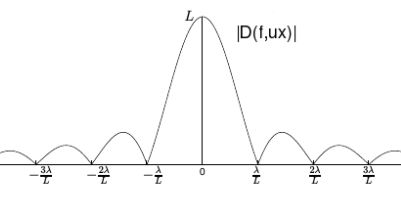
\includegraphics[width = 8cm]{FIGURAS/directividad_apertura.JPG}
	\caption{Directividad apertura}
	\end{figure}
	
	 Se puede apreciar que actúa como un filtro espacial (fenómeno clave para hacer beamforming), diferenciándose claramente el lóbulo principal de los demás, menos directivos.
	 
	 Un array de sensores es, básicamente, una apertura conformada por un número de aperturas lineales, simulando de esta manera el comportamiento de una apertura lineal de longitud la suma de las longitudes de los elementos del array más la separación entre ellos. En la Figura 1.2 se puede observar un array lineal uniforme orientado sobre el eje $z$. Variando la longitud del array con una longitud de onda fija, se pueden lograr diferentes patrones de directividad, como son el ''endfire'' (con el máximo de directividad en 0º y 180º) y el ''broadside'' (con el máximo de directividad en 90º)
	 \begin{figure}[hbtp]
	 \centering
	 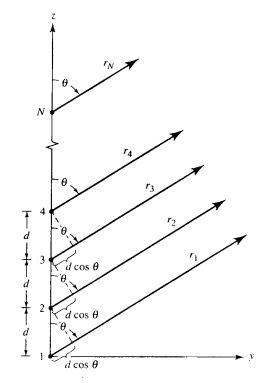
\includegraphics[width = 5cm]{FIGURAS/array_elementos.JPG}
	 \caption{Agrupación de elementos}
	 \end{figure}
	 
A continuación, se ha hecho una pequeña simulación en el programa \textit{FEKO} para un array uniforme lineal de 6 elementos orientado en el eje z, así como la \textit{Figura 1.2}. Cada elemento se ha supuesto un dipolo infinitesimal y con una distancia entre elementos de $\lambda / 2$ para evitar máximos adicionales en el diagrama de radiación y que sea lo más ideal posible.

Si fuese necesario obtener el máximo de radiación de forma perpendicular, lo que se ajusta a los requisitos conforma una agrupación de tipo ''broadside'' ya que, como se ha mencionado, el máximo de directividad se alcanza en $3 \pi / 2$ o en 90º. Mencionado esto, se procede a mostrar los resultados de la simulación a niveles de campo lejano:
\begin{figure}[hbtp]
\centering
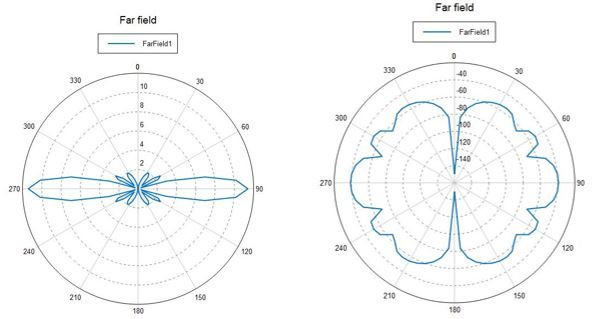
\includegraphics[width = 12cm]{FIGURAS/broadside.JPG}
\caption{Diagrama de radiación broadside}
\end{figure}

Se aprecia que los máximos de radiación se encuentran en 270º y 90º. Cabe destacar que el ángulo en el que se ha hecho el barrido es $\theta$, ya que el array está orientado en el eje z y que el diagrama de la izquierda está expresado el campo en electrón-voltios y el campo de la derecha está expresado en dBV.

Para finalizar la simulación, se adjunta también una representación 3D en la\textit{ Figura 1.4} de la ganancia, sabiendo que la ganancia de una antena está estrechamente relacionada con la directividad de la forma:
\begin{equation}
G = D * \eta_{r}
\end{equation}
Donde $\eta_{r}$ define las pérdidas entre potencia incidente y potencia radiada. Para el caso que interesa, se han impuesto condiciones ideales, por lo que no habrá pérdida alguna y la directividad se corresponde con la ganancia. 
\begin{figure}[hbtp]
\centering
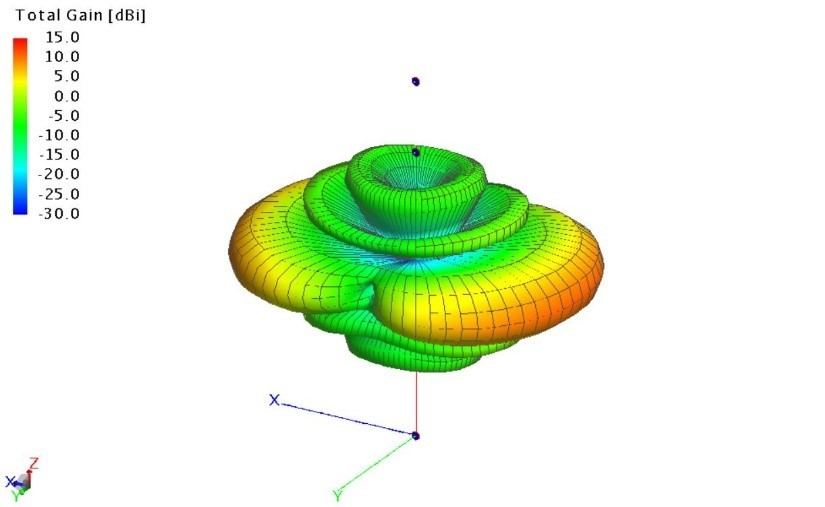
\includegraphics[width = 12cm]{FIGURAS/ganancia_broadside.jpg}
\caption{Ganancia en broadside}
\end{figure}

Se comprueba en este diagrama también el patrón de radiación perpendicular de la agrupación de dipolos infinitesimales desde el punto de vista de la ganancia.

	 
	 El tipo de array que se va a tratar en el proyecto será un array Ad-Hoc de smartphones. No van a realizar una radiación activa como lo simulado con los dipolos infinitesimales, sino que conformarán un array de sensores, los cuales captarán señales acústicas entrantes. Sin ambargo, ha sido de interés incluir esta introducción de antenas activas, ya que el comportamiento será bastante similar y ayuda a entender mejor los diagramas directivos próximos.
	 
	  Las agrupaciones de micrófonos consisten en un número de micrófonos los cuales se combinan para filtrar espacialmente las ondas acústicas. La configuración geométrica del array permitirá filtrar las señales deseadas para diversas aplicaciones. Este filtrado espacial sigue normalmente algoritmos de beamforming, los cuales se detallan en la siguiente sección. Sin embargo, para llegar al filtrado espacial, las señales captadas por los smartphones deben estar sincronizadas. Esto puede ser un problema, ya que el retardo producido desde que el primer móvil recibe la orden de grabar hasta que el último móvil recibe esta orden puede ser determinante. Además, las relojes de los móviles no se encuentran perfectamente sincronizados, por lo que se tendrá que implementar algún algoritmo de sincronización para mitigar estos efectos y llegar a realizar los filtros espaciales adecuadamente.
	 
	\section{Concepto de Beamforming}
	El concepto de ''Beamforming'' agrupa las técnicas necesarias para la determinación de filtros específicos, los cuales tienen el fin de obtener un patrón de directividad con una forma y dirección determinadas.
	
	Un ''beamformer'' se interpreta como un procesador, utilizado conjuntamente con una serie de sensores, para proporcionar una forma versátil de filtrado espacial. El objetivo es estimar la señal procedente de una dirección deseada, en un entorno ruidoso y en presencia de señales de interferencia. El ''beamformer'' actúa de forma similar a un filtro espacial, separando las señales que han sufrido una superposición en frecuencia, pero que se han originado en diferentes localizaciones espaciales. Para determinar el patrón de directividad deseado se hace uso de filtros o, siguiendo la nomenclatura de la sección de procesamiento de señales multicanal, pesos. Estos filtros o pesos se componen de una parte real y de una parte imaginaria.
	\begin{equation}
	w_{n}(f) = a_{n} e^{j\varphi_{n}(f)}
	\end{equation}
	La \textit{ecuación 1.5} se corresponde con un esquema típico de amplitud ($a_{n}$) y fase ($e^{j\varphi_{n}(f)}$). La amplitud determina la forma del patrón de directividad, mientras que la fase interviene en la orientación del lóbulo principal en un determinado ángulo.
	
	El caso que se planteará en este proyecto corresponde a un beamforming acústico. Dentro de este caso, existen dos ramas principales: una relacionada con la extracción de la señal y otra relacionada con la localización de las fuentes sonoras.
		\subsection{Tipos de Beamformers}
		
		Antes de entrar en detalle en los distintos modelos, cabe diferenciar tres tipos de campos de ruido existentes para los cuales sería más adecuado el uso de un tipo de beamformer u otro y el criterio que se va a seguir para evaluarlos:
		\begin{itemize}
		\item Campo de ruido coherente: El ruido se propaga en una determinada dirección con la misma energía.
		\item Campo de ruido incoherente: La correlación de las contribuciones ruidosas es aleatoria.
		\item Campo de ruido difuso: La propagación del ruido es en todas las direcciones con una misma energía.
		\end{itemize}
		
		Se define la ganancia del array como el cociente de la SNR a la salida y la SNR a la entrada del beamformer.
		
		\begin{equation}
		G(f) = \frac{SNR_{o}(f)}{SNR_{i}(f)}
		\end{equation}
		
El factor de directividad (\textit{ecuación 1.7}) se entiende como el cociente del patrón de directividad en la dirección deseada y el patrón de directividad de todas las direcciones en general.

\begin{equation}
F_{d}(f, \phi_{s}, \theta_{s}) = \frac{|D(f, \phi_{s}, \theta_{s}|^{2}}{\frac{1}{4 \pi} \int_{0}^{2\pi}\int_{0}^{\pi}|D(f, \phi, \theta|^{2} sin(\theta) d\theta d\phi}
\end{equation}
		
				Se va a explicar tres clases distintas de beamforming: Beamforming Delay \& Sum, Beamforming MVDR y Beamforming superdirectivo.
		\subsubsection{Delay \& Sum}
		Este primer beamformer es el más comúnmente utilizado en procesos de beamforming debido a simplicidad y a su robustez. El beamformer Delay \& Sum o \textit{DAS} ha sido utilizado en muchos estudios de localización de ruido en aeronáutica, como se verá posteriormente.
		
		En el beamformer DAS, los pesos son representados mediante \textbf{retardos}. Siguiendo la estructura de la \textit{ecuación 1.5} resultaría:
		\begin{equation}
		w_{n}(f) = e^{j \omega t_{n}} / N
		\end{equation}
		Con una contribución uniforme para cada elemento de $1/N$ y siendo $t_{n} = \varphi_{n}(f) / \omega$. Se desea modificar el patrón de directividad de la \textit{ecuación 1.1} hacia una dirección deseada $u_{s}$. Introduciendo el peso obtenido en la \textit{ecuación 1.8} operando con las exponenciales y sacando factor común, el patrón de directividad queda de la forma:
\begin{equation}
		D(f, u-u_{s}) = \frac{1}{N} \sum_{n = 0}^{N-1} e^{2\pi f j (\frac{u r_{n}}{c} - t_{n})}
		\end{equation}		
		Donde $r_{n}$ es el vector de posición del elemento $n$. El objetivo es obtener el patrón de directividad en la dirección deseada $u_{s}$, por lo que fijando $t_{n} = \frac{u_{s} r_{n}}{c}$ conseguimos el direccionamiento comentado. Definimos instante de llegada de la señal justo en la dirección deseada ($u = u_{s}$) como $\tau_{n,s} = -t_{n}$. 		
		
		Los pesos o filtros correspondientes a los $N$ elementos del array del beamformer DAS son:
		\begin{equation}
		\textbf{w}(f) = \frac{1}{N} (e^{j \omega t_{0}},...,e^{j \omega t_{N-1}})^{T} = \frac{1}{N} \textbf{d}(f,u_{s})
		\end{equation}
		Siendo $\textbf{d}(f,u_{s})$ el llamado \textit{steering vector.}

		Básicamente, el beamformer DAS hace la sumatoria de todas las versiones retardadas y de sus correspondientes pesos para cada elemento o micrófono, consiguiendo una superposición destructiva para aquellas señales que no lleguen en la dirección deseada y se conseguirá una superposición constructiva para las señales procedentes de la dirección deseada. Se logra de esta manera un realzamiento de la señal procedente de la fuente de interés, mientras que se suprime la contribución de otras fuentes desde una dirección diferente a la determinada. Además de atenuar las señales procedentes de direcciones distintas a la de interés, este beamformer tiene la capacidad de suprimir la contaminación producida por ruido desde la señal de interés.
		
\textbf{		El beamformer DAS maximiza la \textit{ecuación 1.6} en un campo de ruido incoherente.} Por otra parte, aunque el beamformer DAS mantiene un buen comportamiento ante ruido blanco, el factor de directividad que posee no es muy alto.
		
		\subsubsection{MVDR}
		El principal objetivo del beamformer MVDR (\textit{Minimum Variance Distortionless Response}) es hacer mínima la contribución del ruido, como su nombre indica.
		
		Considerando una señal deseada y el ruido capturado, en el dominio de la frecuencia se obtiene la señal:
		\begin{equation}
		\textbf{X}(f) = S(f)\textbf{d}_{s}(f) + \textbf{V}(f)
		\end{equation}
	Se conoce que, la respuesta del array, apoyándose en la definición de patrón de directividad de la \textit{ecuación 1.1} es el siguiente:
	\begin{equation}
	Y(f) = D(f,u) S(f) = \textbf{w}^{H}(f) \textbf{X}(f) = \textbf{w}^{H}(f)(\textbf{d}_{s}(f) S(f) + \textbf{V}(f))
	\end{equation}
	Donde $\textbf{V}(f)$ es la contribución del ruido.
	
	El beamformer MVDR consta en minimizar la contribución del ruido, por lo que se debe resolver un problema de optimización, imponiendo $w^{H} d_{s}(f) S(f) = S(f)$. Se debe minimizar el error cuadrático medio estimando la correlación del ruido entre canales y la matriz de correlación espacial del ruido.
	
	En canales multitrayectoria, el beamformer MVDR se emplea como un ecualizador, el cual filtra espacialmente las señales deseadas e intenta eliminar lo máximo posible las fuentes de ruido.
	
	Teóricamente, el beamformer MVDR es capaz de mejorar siempre la SNR de una señal de interés captada por el sensor de referencia.
	
	\textbf{		El beamformer MVDR maximiza la \textit{ecuación 1.6} en un campo de ruido coherente.}
	
	\subsubsection{Superdirectivo}
	Este tipo de beamformer es conocido por alcanzar un valor alto en el factor de directividad. Sin embargo, es extremadamente sensible ante patrones de ruido no correlados, como puede ser el ruido blanco y ante pequeños errores en los elementos del array. Frente a ruido blanco, el beamformer superdirectivo además de realzar la señal de interés, amplificaría también el ruido blanco. Se puede entender como un filtro lineal.
	
	\textbf{		El beamformer superdirectivo maximiza la \textit{ecuación 1.6} en un campo de ruido difuso.}
	
	\section{Impacto en la actualidad}
	El procesamiento de señales multicanal tiene múltiples aplicaciones. Algunas de ellas son: radioastronomía, radar, sismología, tomografía, comunicaciones inalámbricas, sonar y tratamiento de audio. Se explicará brevemente la actuación de este tipo de procesamiento para las comunicaciones celulares y para un punto de vista acústico.
		\subsection{Comunicaciones Inalámbricas}
		Las comunicaciones celulares en la actualidad emplean sectorización por células para proporcionar más frecuencias por área de cobertura.
		\begin{figure}[hbtp]
		\centering
		\includegraphics[width = 8cm]{FIGURAS/sectorización.JPG}
		\caption{Sectorización celular}
		\end{figure}
		
	
	Sin embargo, esta sectorización no fue suficiente para abarcar el creciente número de usuarios que solicitan recursos de frecuencia, por lo que, en la última generación estandarizada de comunicaciones móviles (4G), se emplearon técnicas ''MIMO'' y ''Smart Antennas. MIMO es un acrónimo que se refiere a ''Multiple Input Multiple Output'', por lo que se podrá utilizar una agrupación de antenas tanto en el emisor como en el receptor. Se puede entender mejor el concepto observando el canal del sistema correspondiente a la \textit{Figura 1.2}. En concreto, es un canal MIMO 4x4.
		
		Debido al uso de múltiples antenas, se pueden emplear las técnicas de multiplexado espacial y diversidad espacial. La primera de ellas consigue mejorar la ganancia mediante la transmisión de distintos flujos de información independientes a través de las múltiples antenas. Esto implica un aumento considerable de la tasa de bits respecto a los sistemas con una única antena. Con la diversidad espacial se incrementa la ganancia en codificación mediante la transmisión de secuencias redundantes por varias antenas.
		
		\begin{figure}[hbtp]
		\centering
		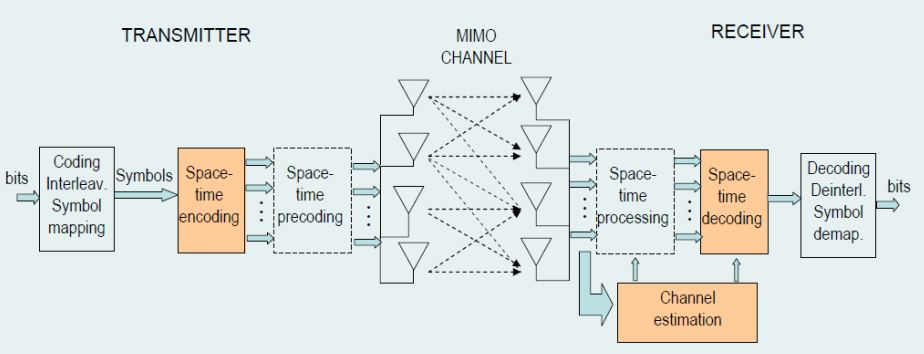
\includegraphics[width = 10cm]{FIGURAS/sistema_MIMO.JPG}
		\caption{Sistema MIMO}
		\end{figure}

		En referencia a la introducción de las llamadas ''Smart Antennas'', son capaces de adaptar el patrón del haz de radiación con el propósito de mejorar la calidad de la señal deseada y minimizar el impacto de la señal interferencia. Esta adaptación implica el uso de beamforming. El beamformer puede ser adaptativo, el cual dirige el haz principal hacia la señal de interés, o conmutado, el cual posee una serie de patrones de radiación fijos. Este fenómeto es levemente ilustrado en la \textit{Figura 1.3}.
		\begin{figure}[hbtp]
		\centering
		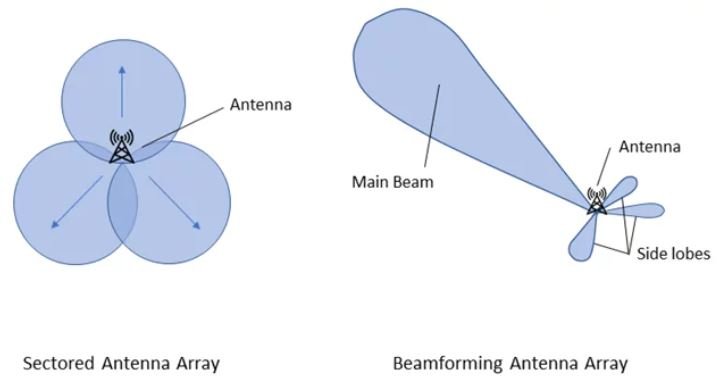
\includegraphics[width = 8cm]{FIGURAS/beamformer_adaptativo.JPG}
		\caption{Beamforming en comunicaciones inalámbricas}
		\end{figure}
		
		\subsection{Procesamiento acústico}
		En referencia un punto de vista acústico y manipulación de audio, se van a exponer dos técnicas distintas. La primera será diarización de locutores y la segunda será la localización de fuentes sonoras.
			\subsubsection{Diarización}
			La diarización entre locutores consiste en determinar los instantes de tiempo en los que cada locutor interviene, dada una señal de audio captada con array de micrófonos, como va a ser el caso. Se expone el ejemplo real de una sala de reunión con múltiples locutores y múltiples micrófonos distribuidos en la sala. Para aprovechar la capacidad de un array de múltiples micrófonos, se pueden utilizar técnicas de beamforming, ya explicadas en una sección anterior para realzar la señal de interés.
			
			Antes de ningún proceso que abarque a todos los micrófonos, se debe aplicar un filtro de Wiener a cada canal individual para eliminar el ruido aditivo. Teniendo en cuenta el tiempo de llegada de cada señal y el número total de micrófonos, se implementa un algoritmo que implica correlación cruzada entre señales, obteniendo de esta manera el canal que proporciona una mejor calidad de señal. Tras aplicar beamforming, computando los retrasos entre cada canal, se propone usar el algoritmo de Viterbi, el cual se encarga de hallar el camino o secuencia con mayor probabilidad. El objetivo de este último paso es proporcionar una continuidad a la señal del locutor que está en ese momento hablando, estableciendo el retardo de la señal y filtrando la dirección del haz no deseada.	
			\begin{figure}[hbtp]
			\centering
			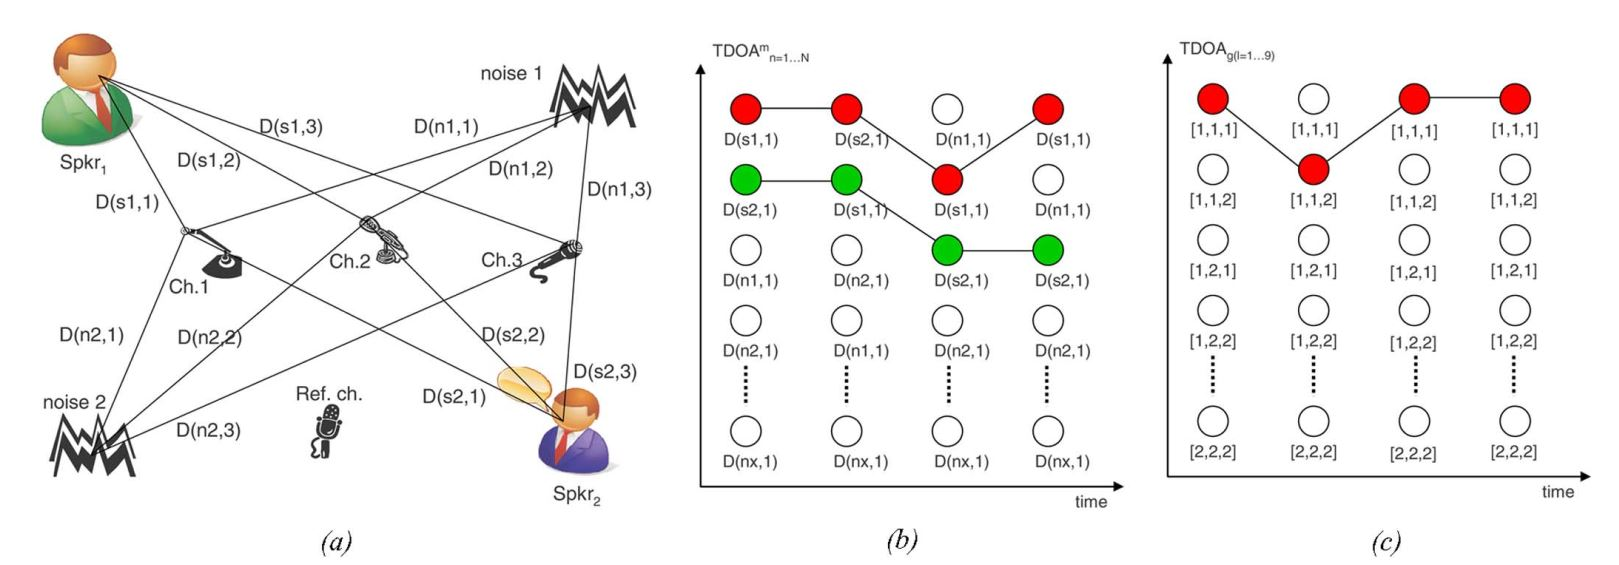
\includegraphics[width = 13cm]{FIGURAS/diarizacion.JPG}
			\caption{Decodificación de Viterbi}
			\end{figure}	
			
			En la \textit{Figura 1.4} se esquematiza el algoritmo de Viterbi para un ejemplo de dos locutores, dos fuentes de ruido y micrófonos distribuidos. En el primer paso (b) para cada canal individual, se obtiene los dos mejores caminos en función del tiempo. En el segundo paso (c) se seleccionan los retardos apropiados, considerando todas las posibles combinaciones de todos los canales. Se acaba eligiendo el mejor camino según los datos de distancias y correlación.\linebreak 
			\textit{Nota: Las columnas de la representación trellis del algoritmo de Viterbi corresponden a la diferencia de tiempos de llegada obtenidos anteriormente.
}
			\subsubsection{Localización de fuentes}
			Técnicas de beamforming acústico son usadas para el propósito de localizar fuentes sonoras. Hay que destacar que, las condiciones ambientales pueden afectar considerablemente a la fiabilidad del beamforming. La reflexión y difracción del las ondas sonoras dan lugar a las llamadas ''fuentes fantasma'' o \textit{ghost sources}. Estas \textit{ghost sources} aparecen cuando el proceso de beamforming no está perfectamente adecuado para los fenómenos de propagaciones reales del entorno.
			
			
			\begin{itemize}
				\item[-] Una aplicación interesante de beamforming es la relacionada con la identificación de fuentes en movimiento. En este caso, se debe considerar el efecto Doppler, por lo que se tendrá que compensar este fenómeno. El beamforming aplicado a objetos en movimiento se suele aplicar en el dominio del tiempo, ya que es más rápido para un número grande de micrófonos. Con las coordenadas del móvil estimadas y la frecuencia Doppler compensada, se procede con un beamforming ''delay and sum'', visto en secciones anteriores.
				\item[-] Un campo en el que el beamforming ha supuesto una herramienta de mejora importante es en los experimentos llamados ''Túneles de viento'' o \textit{Wind tunnels}. Estos experimentos se realizan con el propósito de analizar el efecto del aire incidente en objetos. Se simula una situación real, enfocando una estructura como puede ser un avión, una aeronave o incluso edificaciones. 
			\begin{figure}[hbtp]
			\centering
			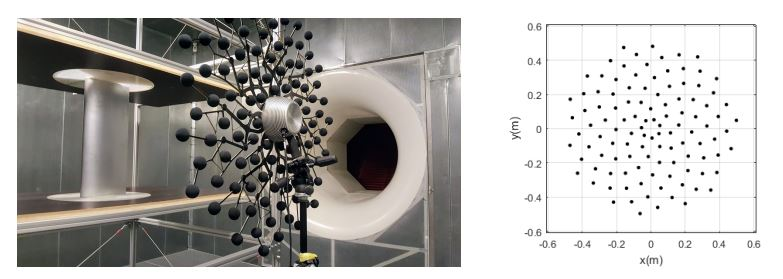
\includegraphics[width = 12cm]{FIGURAS/wind_tunnel.JPG}
			\caption{Configuración del array para un túnel de viento}
			\end{figure}
			
			Las ondas de sonido radiadas por las fuentes aero-acústicas ubicadas en la superficie del modelo, sufren refracción y scattering debido a entorno del experimento, por lo que deberá existir un algoritmo para compensar este fenómeno. La técnica de beamforming juega un papel importante al estimar las repercusiones acústicas que sufre el modelo y evitar posibles averías o incluso conseguir una mejoría en el comportamiento del modelo. En la \textit{Figura 1.5} se muestra el experimento real (parte de la izquierda) y la disposición de los micrófonos (parte de la derecha).
				\item[-] Por último, mencionar la aplicación de beamforming en interiores. Micrófonos empotrados son normalmente utilizados en entornos de interios, así como cabinas de avión o interiores de automóviles. De esta manera, se consigue identificar la ubicación de las fuentes sonoras y actuar frente a estas.
			\end{itemize}
			
	
	\section{Justificación del proyecto}
	\section{Distribución del proyecto}
		\subsection{Requisitos de realización}
		\subsection{Seguimiento del proyecto}
		Aquí va una lista de lo que he hecho: servidor, app y algoritmo.
		\subsection{Entornos de trabajo}
		Java, AndroidStudio, Python...
\chapter{Planteamiento del problema}

\chapter{Desarrollo del servidor externo}
	Tal y como se ha comentado, para crear la comunicación con los móviles y manejar las distintas órdenes correspondientes al objetivo de grabar de forma coherente en cada dispositivo, es necesaria la incorporación de un servidor externo.
	
	
		\section{Propósito principal}
			Lo primero, es aclarar la función que el servidor externo va a desempeñar. Su función será dar órdenes a la aplicación así como las de comienzo y finalización de la grabación. Además, será el encargado de, una vez recibidas las grabaciones procedentes de la aplicación, guardar los ficheros correspondientes. Por supuesto, será el encargado de habilitar un puerto disponible para cada dispositivo que se conecte.
			
			
			\subsection{Requisitos funcionales}
				A continuación se van a enumerar los parámetros funcionales a nivel de software que posee el servidor externo creado.
				
				\begin{itemize}
				\item Capacidad para manejar un número máximo de 10 clientes.
				\item La primera conexión de cada cliente se realiza en un mismo puerto común.
				\item Una vez realizada la primera conexión, el servidor maneja los puertos de conexión fija de los clientes, buscando puertos libres, de manera que tengan una asignación consecutiva (ej: nº puerto 5001, 5002, 5003...)
				\item Una vez conectados el número de clientes especificado, esperará la confirmación de la aplicación para enviar la orden de ''comenzar a grabar''
				\item Se le podrá especificar la duración de la grabación en milisegundos.
				\item Una vez acabada la grabación por cada uno de los clientes, se guarda cada fichero de audio en formato de datos brutos (.raw) con la nomenclatura: ''Device'' + ''nº cliente''
				\item El servidor muestra por pantalla las marcas de tiempo correspondientes al inicio y al final de la grabación de cada dispositivo o cliente.
				\item Posee una función la cual reproduce una señal de sincronización una vez hayan comenzado a grabar todos los dispositivos.
				\end{itemize}
			
			\subsection{Requisitos no funcionales}
			En esta parte se va a exponer la calidad del software en sí mismo, con motivo de evaluar su funcionamiento.
			\begin{itemize}
			\item Es necesario especificar el número de conexiones o número de dispositivos que se van a conectar antes de iniciar el servidor.
			\item Una vez iniciado el servidor, espera indefinidamente (timeout) hasta que se realicen el número de conexiones especificadas.
			\item Los tiempos correspondientes a la comunicación entre los diversos dispositivos y el servidor son variables.
			\item Si a la hora de grabar se produce algún problema en uno de los dispositivos, los ficheros correspondientes a los demás dispositivos se guardarán correctamente, mientras que el fichero correspondiente al dispositivo erróneo, no se almacenará de forma correcta.
			\item Los tiempos de respuesta del servidor dentro de una zona de cobertura local rondan los 100 milisegundos.
			\item La comunicación del servidor con los distintos clientes, no se produce de una forma simultánea, sino que genera y recibe información de los dispositivos de uno en uno.
			\item Las marcas temporales devueltas por el servidor son relativas, ya que dependen de la sincronización de los relojes de cada dispositivo en concreto.
			\item Si se desea un tiempo de grabación alto, se deberá aumentar el ''buffer'' correspondiente al amacenamiento de bytes de los archivos de grabación.
			\end{itemize}
		
		\section{Construcción del servidor}
		
			Como ya se ha comentado anteriormente, para la implementación del servidor se ha utilizado el entorno de ''NeatBeans'' debido a la facilidad que proporciona el lenguaje de programación ''java'' con los \textit{sockets} para la comunicación cliente-servidor.
			
			Se va a proporcionar una noción respecto al concepto de \textit{socket} y la típica comunicación cliente-servidor. Acto seguido se verá en detalle cada funcionalidad implementada en el servidor	.
			
			\subsection{Noción general y noción de \textit{socket}}
				Para entender el manejo de los sockets, es necesario conocer la comunicación estándar cliente-servidor.
				
				En una comunicación vía red, la información se desglosa en paquetes. La forma en la que están estructurados estos paquetes, la define el protocolo de transporte utilizado. En el caso que nos concierne, debido a que tenemos el propósito de entablar una comunicación orientada a conexión, se va a utilizar el protocolo TCP (Transfer Control Protocol), complementado con IP (Internet Protocol), formando TCP/IP. Este protocolo utiliza dos piezas claves de identificación: la dirección IP y un número de puerto.
				
				Los términos que hacen referencia a los conceptos de \textit{cliente} y de \textit{servidor} son que el cliente debe iniciar la comunicación, mientras que el servidor espera pasivamente a este primer mensaje por parte del cliente; una vez recibe el servidor el mensaje del cliente, el servidor responde de forma coherente a la petición.

				\begin{figure}[hbtp]
				\centering
				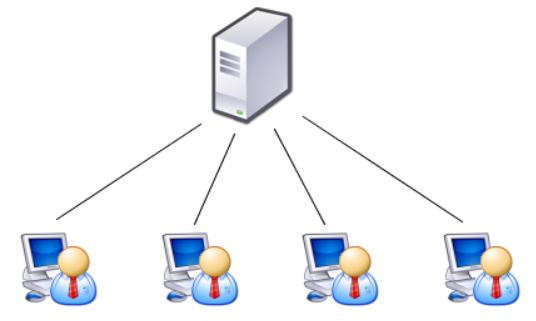
\includegraphics[width = 7cm]{FIGURAS/cliente-servidor.JPG}
				\caption{cliente-servidor}
				\end{figure}
				
				 La distinción \textit{cliente-servidor} es importante porque el cliente necesita conocer la dirección IP y el puerto del servidor, pero no viceversa.
				 
				 En concepto de socket es abstracto. Se puede entender como un método el cual permite la comunicación de aplicaciones en una misma red, pudiendo enviar y recibir datos a través del socket. El protocolo TCP/IP permite transmitir flujos de datos y a través de un socket, una aplicación es capaz de alcanzar un puerto disponible de la red. En la Figura 3.2 se esquematiza la posición de los sockets en el entorno de comunicación.
				 \begin{figure}[hbtp]
				 \centering
				 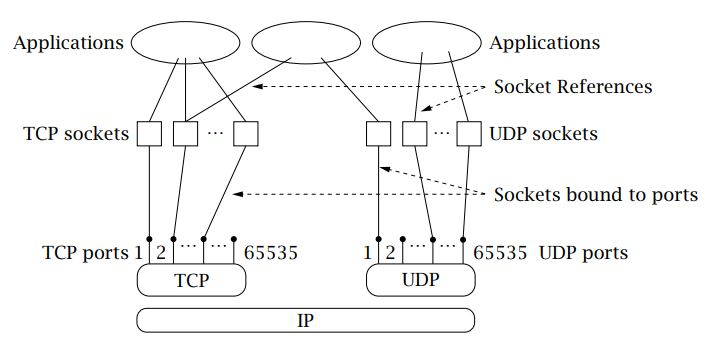
\includegraphics[width = 10cm]{FIGURAS/Explica_Sockets.JPG}
				 \caption{TCP sockets}
				 \end{figure}	
		El manejo de los sockets en Java lo podemos encontrar en su propia API. 
		\begin{description}
				 \item[Server Socket y Socket:] Se deben inicializar tanto los sockets correspondientes al cliente como los correspondientes al servidor. El socket del servidor o ''Server Socket''  hace referencia al puerto al que debe conectar el cliente para mantener la comunicación con el servidor. El socket perteneciente al cliente o ''Socket'' es el cual se le asigna al cliente por el servidor una vez el cliente haya enviado una request ó petición  mediante el Server Socket. El socket del cliente es de utilidad al propio servidor para manejar al cliente correspondiente y para inicializar este último se necesita además del número de puerto, la dirección IP del servidor.
				 
				 En java, el socket procedente al servidor se inicializa de la siguiente manera:
				 \begin{center}
				 \textit{ServerSocket server = new ServerSocket(Port)}
				 \end{center}
				 El socket correspondiente al cliente:
				 \begin{center}
				 \textit{Socket client = new Socket(IP, Port)}
				 \end{center}
				 
				 \item[InputStream y OutputStream:] La comunicación se realizará mediante flujos de entrada y de salida o también llamados \textit{InputStream} y \textit{OutputStream}. Para transmitir datos en forma de byte, más en específico, se utilizan los flujos \textit{DataOutputStream} y \textit{DataInputStream}. Se corresponden al flujo de salida y al flujo de salida respectivamente. Desde el punto de vista del servidor, el \textit{DataInputStream} va del cliente al servidor y el \textit{DataOutputStream} va del servidor al cliente.
				 
				 La sintaxis en java para inicializar estos puentes es la siguiente:
				 \begin{center}
				 \textit{DataOutputStream  output = new DataOutputStream(client.getOutputStream())}
				 
				 \textit{DataInputStream  input = new DataOutputStream(client.getInputStream())}
				 \end{center}
				 En la salida (\textit{output}) se escribirán bytes para ser enviados y en la entrada (\textit{input}) se leerán los bytes entrantes, valga la redundancia.
				 \end{description}	
				 
				 Teniendo una idea general de los que es un socket y cómo se utiliza, es trivial que en la aplicación a cual se comunica con el servidor poseerá sockets relacionados con el dispositivo en cuestión, para comunicarse correctamente con el servidor y su correspondiente puerto.
				 
				 \subsection{Implementación del servidor}
				 Llegados a este punto, se procede a explicar la arquitectura del propio servidor creado para el proyecto.
				 
				 Lo esperado es manejar 10 clientes, por lo que el servidor podrá crear y dirigir 10 sockets de clientes distintos. Aún así, se han determinado dos conexiones. La primera conexión será común para todos los dispositivos, es decir, debido a esta primera conexión se ha creado un socket de servidor y otro socket de cliente adicionales, los cuales serán estáticos a todos los clientes. Esto significa que cada dispositivo, por primera vez, se conectará a un mismo puerto. Una vez conectado el cliente a este puerto inicial, el servidor le proporcionará al cliente un nuevo puerto de conexión fija, en el cual se llevará a cabo el intercambio final de datos.
				 
				 Para la selección de los números de puertos, hay que tener en cuenta cuáles están en uso y cuáles no, para que no haya ningún tipo de problema. Los puertos del 0 hasta el 1023 están reservados para el sistema operativo y los utilizan protocolos como FTP, DNS, SSH... Por lo que, para asegurar una correcta elección de número de puerto, se establece el puerto fijo de la primera conexión en el número de puerto 5000 y los puertos finales serán el 5001, 5002, 5003, ... 5010. 
				 
				 Además, para comprobar la disponibilidad del servidor y el número de puertos abiertos se ha hecho uso del comando \textit{telnet} desde la terminal de Windows. Con este comando se comprueba fácilmente la conexión a un puerto determinado conociendo la dirección IP de destino. La sintaxis del comando es la siguiente:
				 \begin{center}
				 \textit{telnet[dominio ó dirección IP][puerto]}
				 \end{center}
				 Si se llega a entablar la conexión, aparecerá una sección de pantalla vacía indicando que el puerto se encuentra disponible y si la conexión no se establece, se emitirá un mensaje de error lo cual indica que el puerto al que se referencia no está disponible o que, simplemente el servidor no se mantiene en escucha en ese puerto específico.
				 
				 El servidor creado posee varias funciones, las cuales se enumeran y se explican a continuación:	 	 
				\begin{itemize}
				\item \textbf{Search4port}: Función encargada de devolver una lista de puertos disponibles para iniciar nuevas conexiones. Toma de argumentos de entrada un vector del tipo ''booleano'' donde se indica los puertos ocupados.
				\item \textbf{Recording}: Función encargada de enviar la orden de grabar a cada cliente. Una vez el servidor se encuentre en esta función, deberá recibir el ''ACK'' de todos los clientes para lanzar la orden de grabar. Toma de argumentos de entrada los sockets correspondientes al número de clientes.
				\item \textbf{Delay}: Esta función es la manejadora del tiempo de grabación. Simplemente manda a reposar el hilo principal durante un tiempo determinado, introducido en milisegundos.
				\item \textbf{stopRecording}: Como su propio nombre indica, es la función relacionada con el envío de la orden de parar la grabación. Similar a \textit{Recording} con la diferencia de que se envía la orden opuesta y que el servidor no espera ningún ''ACK'' por parte de los clientes para emitir la orden correspondiente.
				\item \textbf{getTimeStamp}: Función que lee la marca de tiempo devuelta por cada móvil. Como argumento de entrada toma el socket de cada cliente, ya que la marca temporal de cada móvil proviene de la aplicación.
				\item \textbf{Time}: Si fuese necesario devolver una marca temporal ''absoluta'', tomada con el reloj del servidor, se puede llamar a esta función cuando se desee sin argumentos de entrada. Puede ser útil para comparar las demás marcas de tiempo ''relativas'' obtenidas para cada dispositivo.
				\item \textbf{timeView}: Se apoya en la función \textit{Time()}. Únicamente muestra la marca de tiempo definida con el servidor por pantalla, para tener constancia del tiempo absoluto en que empieza cada grabación.
				\item \textbf{serverImpulse}: Esta función se encarga de emitir un chirp inicial, justo cuando todos los dispositivos están grabando. De esta manera, con la señal inicial captada, se podrá llegar a un algoritmo de sincronización entre las grabaciones efectivo.
				\item \textbf{playChirp}: Para realizar un método de sincronización distinto al comentado en la función anterior, se puede llamar a esta función para emitir una orden de reproducir una señal ''chirp'' en cada uno de los móviles o clientes mientras se encuentran en estado activo de grabación, con el propósito obtener las señales grabadas sincronizadas.
				\item \textbf{saveFiles}: Por último, se llama a esta función. Su principal cometido es recibir los bytes procedentes de cada una de las grabaciones, almacenarlos en un buffer temporal, y guardarlos en la memoria de la máquina en la que se está ejecutando el servidor. Se debe ser coherente con el tiempo de la grabación y el tamaño del buffer temporal. Guarda las grabaciones como archivos de datos en bruto (.raw). Toma de argumentos de entrada el socket de cada cliente.
				\end{itemize}

				
				
		\section{Comunicación}
		En esta sección se va a documentar en profundidad la comunicación producida entre el servidor y cada uno de los dispositivos.
		
		Antes de nada, se debe tener claro el orden de procedimiento del servidor. Una vez iniciado el servidor, se presentan los siguientes flujos comunicativos:
		\begin{enumerate}
		\item El servidor se queda esperando hasta que recibe una petición de conexión de un cliente al puerto 5000.
		\item Una vez aceptada esta primera conexión, el servidor busca un puerto libre, mediante la función \textit{Search4port} y se lo devuelve al cliente para que realice una nueva conexión.
		\item El cliente envía una nueva \textit{request} al puerto indicado por el servidor. Al aceptar el servidor esta nueva conexión, el cliente finalmente se encuentra en el puerto adecuado para realizar la comunicación completa.
		\item Ya conectados el número de clientes especificado, el dispositivo deberá enviar un mensaje de ''READY'', para dar a entender al servidor que está listo para grabar.
		\item El servidor emite la orden de grabar (''START'') y espera a que cada uno de los móviles le hagan llegar un ''ACK'' de confirmación por empezar a grabar. Adicionalmente, los móviles transmiten al servidor la marca temporal correspondiente al inicio de la grabación y el servidor, por su parte, emite una marca temporal absoluta para cada confirmación recibida, la cual se utilizará más adelante para ayudar a sincronizar las señales.
		\item Pasados los segundos de grabación establecidos, el servidor emite la orden de parar la grabación (''STOP'') y cada dispositivo devuelve de nuevo una marca temporal, relacionada con el final de la grabación.
		\item Por último, cada smartphone envía al servidor el fichero de grabación resultante.
		\end{enumerate}
			
			Con propósito a comprobar este flujo de transporte enumerado, se hará uso de la herramienta \textit{WireShark}. El principal objetivo de esta herramienta es analizar el tráfico de una red. A parte, es ideal para estudiar cualquier tipo de comunicaciones y problemas de red.
			
			Cabe anotar que, tras diversas pruebas, se ha obtenido un resultado más constante respecto a los tiempos de la red si se crea un punto de acceso inalámbrico en la máquina en la que corre el servidor y que todos los smartphones que deseen interactuar con el servidor, deberán conectarse a este punto de acceso creado. La comunicación mediante la Wi-Fi local presentaba muchos retardos inesperados, debido a que diversos dispositivos están conectados a la red, por lo que el tráfico de paquetes será mayor y, lo más desfavorable, con más rango de aleatoriedad.
			Además, disponiendo de un punto de acceso privado, el tráfico de la red se reducirá considerablemente a la hora de visualizar el flujo de transporte.
			
			Se ha filtrado el tráfico de manera que solo se visualice el protocolo TCP en el puerto 5000 y en el puerto 5001, ya que se va a mostrar el flujo de un único dispositivo  para simplificar el intercambio de mensajes. Mencionado esto, se presenta la captura del tráfico correspondiente al punto de acceso inalámbrico. 
			
			El tráfico resultante únicamente del conexionado con el servidor es presentado en la \textit{Figura 3.3}.
			
\begin{figure}[hbtp]
\centering
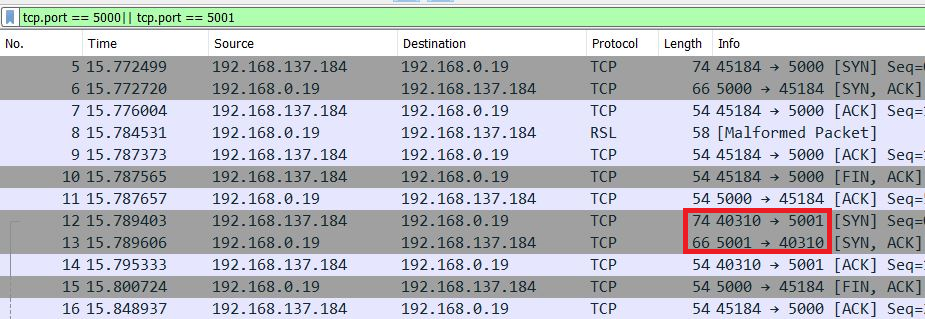
\includegraphics[width = 15cm]{FIGURAS/trafico_connect.png}
\caption{Tráfico ''connect''}
\end{figure}

Se puede apreciar la dirección IP de la máquina donde corre el servidor (192.168.019) y la dirección IP del smartphone (192.168.137.184). Además, se observa enmarcado en rojo dos envíos de paquetes interesantes, ya que es el momento en el cual el servidor le ha enviado ya el siguiente puerto de conexión fija y realiza de nuevo el dispositivo una \textit{request} al nuevo puerto (50001).

 Para entender mejor todos los envíos de paquetes, se ejemplifica en el diagrama UML de la \textit{Figura 3.4} el típico esquema de un flujo TCP. El protocolo TCP utiliza el llamado ''\textit{three-way handshake}'' con el propósito de establecer una conexión fiable. Este método de conexión se basa en el envío y recepción de señales de sincronización y señales de acuse y recibo, o también llamadas \textit{SYNC} y \textit{ACK}. Concretamente, se distribuyen en su envío de la manera:
 \begin{enumerate}
 \item SYN
 \item SYN/ACK
 \item ACK
 \end{enumerate}
Una vez se haya completado el envío y recepción de esos tres mensajes, se podrá confirmar que existe una conexión fiable. El cliente juega un papel activo, el cual empieza enviando un segmento SYN, portador de su número de secuencia. El servidor, por su parte, juega un papel más pasivo.

\begin{figure}[hbtp]
\centering
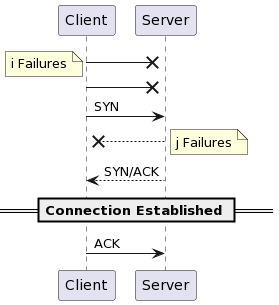
\includegraphics[width = 8cm]{FIGURAS/TCP_flow.png}
\caption{Conexión TCP}
\end{figure}


Al recibir el servidor el segmento SYN, este último responde otro segmento SYN con su número de secuencia inicial y con un acuse y recibo (ACK). De esta manera, conociendo los números de secuencia de cada parte y con el ACK, ayuda a reconocer mensajes erróneos o perdidos. Cuando el cliente recibe el paquete SYN/ACK del servidor, sabe que se ha establecido exitosamente la conexión y devuelve un ACK al servidor para terminar.

En cada fase del proceso, es posible que se produzca una pérdida de paquetes o que no lleguen al destino correctamente, por lo que existe un tiempo límite o \textit{timeout} con el cual se comprueba si se debe enviar de nuevo el segmento de sincronización. Todo este flujo de establecimiento de la conexión, lo podemos apreciar claramente en la \textit{Figura 3.3}. El proceso de conexionado, en este caso, se realiza dos veces (una vez al puerto común 5000 y otra vez al puerto fijo 5001).

Una vez hecho el conexionado, el cliente hace saber al servidor que está listo para grabar. Cuando todos los dispositivos le hayan dado la confirmación para empezar a grabar, el servidor enviará la orden para empezar. Este flujo lo podemos ver en la \textit{Figura 3.5}.

\begin{figure}[hbtp]
\centering
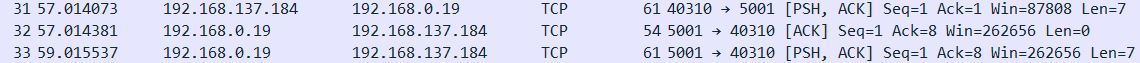
\includegraphics[width = 15 cm]{FIGURAS/trafico_record.JPG}
\caption{Tráfico ''record''}
\end{figure}

Si observamos el contenido del primer paquete y del último paquete del flujo presentado, se pueden apreciar los correspondientes mensajes de ''READY'' por parte del dispositivo y de ''START'' por parte del servidor en la \textit{Figura 3.6}. Los bytes anteriores a las palabras clave comentadas son correspondientes a la cabecera del paquete.

\begin{figure}[hbtp]
\centering
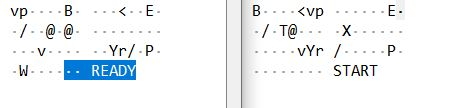
\includegraphics[width = 8 cm]{FIGURAS/startready.JPG}
\caption{Palabras clave comienzo}
\end{figure}

Una vez emitida la orden de grabar por el servidor, cada dispositivo envía un ''ACK'' adicional y empieza la grabación. En el período de tiempo de grabación no se intercambian paquetes, ya que el servidor se encuentra en reposo y los móviles se encuentran grabando.

Cuando la grabación finaliza, llega el momento de intercambiar el archivo de datos brutos almacenado. Este proceso se puede apreciar en la \textit{Figura 3.7}.

\begin{figure}[hbtp]
\centering
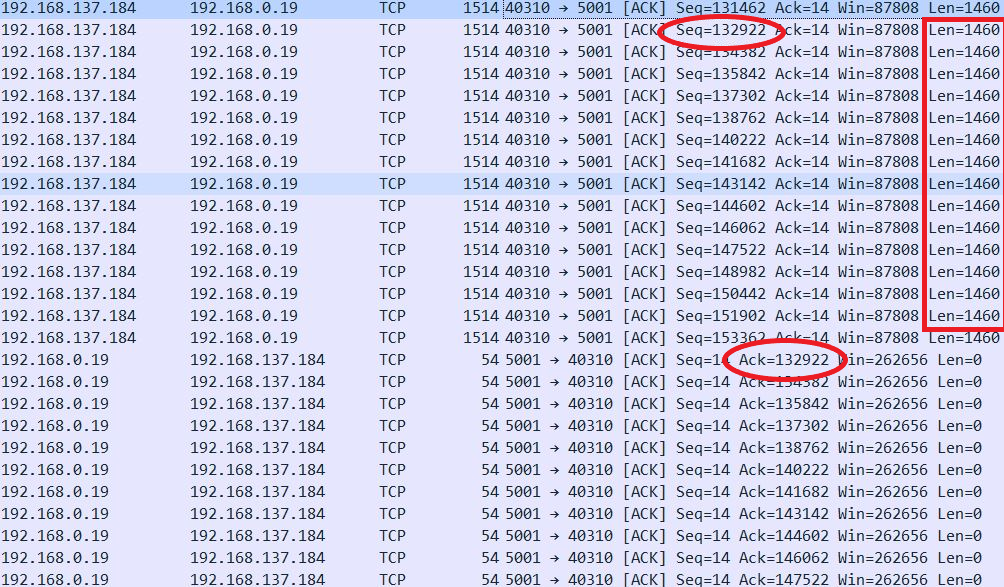
\includegraphics[width = 16 cm]{FIGURAS/intercambio_grabacion.png}
\caption{Transferencia archivo}
\end{figure}

En la que se puede observar que el envío se divide en tramas de 1460 bytes y que llegados una serie de paquetes, el servidor responde con un ACK referenciando al número de secuencia del paquete el cual se está confirmando su correcta llegada.	
				
			Con los datos proporcionados por el tráfico de red, se traza un diagrama UML en la \textit{Figura 3.8} para una mejor visualización de la comunicación entre el servidor y un cliente.
			
	\begin{figure}[hbtp]
			\centering
			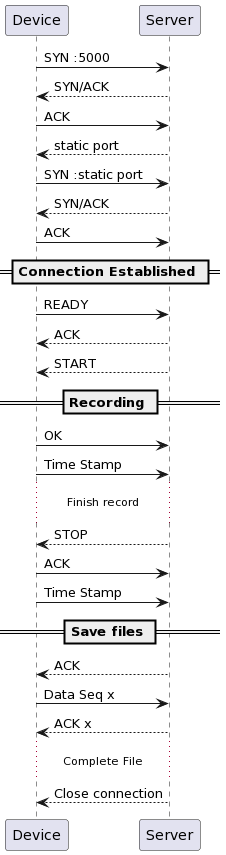
\includegraphics[width = 5cm]{FIGURAS/uml.png}
			\caption{Tráfico completo.}
			\end{figure}
					
			
			
			
			
\chapter{Desarrollo de la aplicación }

Tal y como se ha comentado anteriormente, para la comunicación entre el servidor y los respectivos smartphones y para que cada uno ejecute la grabación correctamente, es necesario la introducción de una aplicación Android en cada uno de los dispositivos. De esta manera se consigue la interconexión que se desea.

	\section{Introducción a la aplicación}
	La aplicación ha sido desarrollada en \textit{Android Studio}. Se le ha especificado el nombre de \textit{BeamRec}.
	
	El propósito de la aplicación es cumplir los requisitos necesarios, esto es la conexión con el servidor, la correcta grabación y la debida transmisión del fichero de grabación. La interfaz de la aplicación está pensada para que sea lo más intuitiva posible, para conseguir únicamente la meta del proyecto que se está tratando.
	
	Nada más abrir la aplicación, la interfaz resultante se muestra en la \textit{Figura \ref{interfaz1}}. Como se puede apreciar, directamente proporciona la opción al usuario de conectar el dispositivo con el servidor externo. Una vez se pulse el botón de ''CONNECT'', el cliente enviará una petición de conexión al servidor especificado.

\begin{figure}
 \centering
  \subfloat[]{
   \label{interfaz1}
    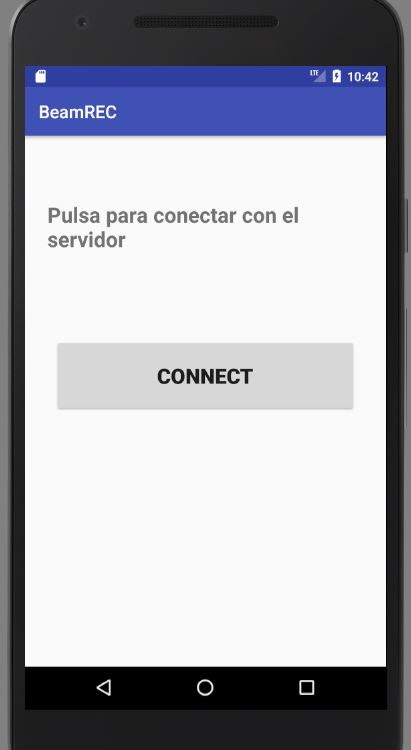
\includegraphics[width = 5 cm]{FIGURAS/interfaz1.JPG}}
  \subfloat[]{
   \label{interfaz2}
    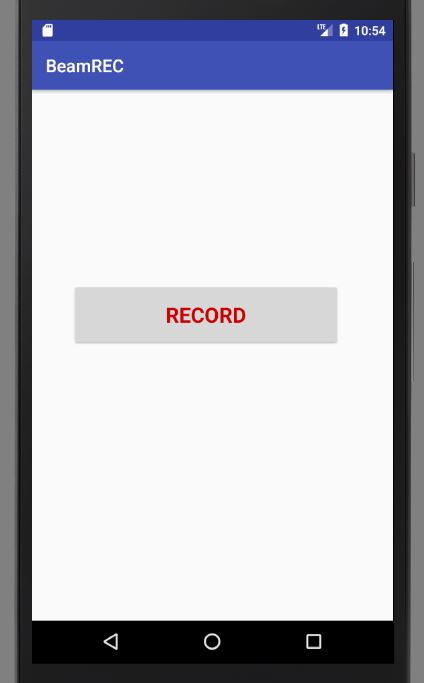
\includegraphics[width=5cm]{FIGURAS/interfaz2.JPG}}
 \caption{Interfaces de la aplicación}
\end{figure}


	
	Al pulsar el botón de ''CONNECT'' y habiéndose conectado el dispositivo exitosamente al servidor, la siguiente interfaz o \textit{activity} que el usuario visualiza se observa en la \textit{Figura \ref{interfaz2}}.
	
	En este caso, la aplicación únicamente proporciona la opción de grabar. Este botón se deberá pulsar una vez todos los móviles que se desean conectar al servidor hayan conseguido una conexión exitosa. Cuando se desee comenzar a grabar, una vez pulsado el botón, el cliente envía el correspondiente mensaje de que está listo para grabar hacia el servidor. Este último recibe el mensaje y emite la orden de grabar. Si se desea repetir la grabación, se deberá realizar desde el principio el proceso de conexión con el servidor externo. Será necesario que cada uno de los móviles estén conectados a la misma red a la que está conectado el servidor.

	\section{Funcionalidades}
	En esta parte se va a explicar las distintas funciones internas de la propia aplicación.
	
	En total, se han creado 3 clases java en Android Studio:
	\begin{itemize}
	\item \textbf{MainActivity}: Es la clase principal. En ella se encuentra el diseño de la primera interfaz mostrada en la \textit{Figura 4.1}. Al pulsar el usuario el botón, se hará una llamada a la siguiente clase con su nueva interfaz.
	\item \textbf{RecordClient}: Contiene el diseño de la segunda interfaz de la aplicación (\textit{Figura 4.2}). Esta clase es la encargada de mantener la conexión con el servidor dada una dirección IP específica y el puerto común, el cual se ha determinado como el puerto número 5000 en la sección del servidor. Realiza todo el proceso de doble conexión al servidor en segundo plano y, una vez conectado el dispositivo al servidor, se cargará la interfaz correspondiente a la acción de grabar.
	
	Al pulsar el usuario el botón de ''RECORD'', se mandará el mensaje de ''READY'' al servidor y se esperará a la orden de empezar la grabación emitida por el servidor. La comunicación con el servidor desde la aplicación se realiza de manera similar que en el servidor: con el uso de \textit{Sockets} y flujos de datos \textit{DataInputStream} y \textit{DataOutputStream}. Cuando la aplicación recibe la orden de grabar por el servidor, se hace la llamada a la clase \textit{Recorder} y empieza la grabación en un nuevo hilo. En el hilo principal se procede al envío del ''ACK'' y de la marca de tiempo correspondiente al comienzo de la grabación por parte del dispositivo al servidor y se mantiene en espera hasta recibir la orden correspondiente a parar la grabación.
	
	Una vez recibida la orden de ''STOP'' procedente del servidor para parar la grabación, se hace la llamada correspondiente a la clase Recorder para dejar de grabar y se envía la marca de tiempo de finalización. Acto seguido, se procede a la manipulación del archivo. Mediante las clases \textit{BufferedInputStream} y \textit{BufferedInputStream} se almacenará la grabación en un buffer momentáneo que será enviado directamente al servidor.
	
	Cabe destacar que, en esta clase también se definen los permisos necesarios para la correcta ejecución de la aplicación en el dispositivo Android. Estos son los permisos de utilización del micrófono y de la grabadora del smartphone.
	
	\item \textbf{Recorder}: Esta clase, como se ha mencionado en \textit{RecordClient}, es la responsable de la propia acción de grabar. Se ejecuta en segundo plano y es capaz de ejecutar una grabación con una frecuencia de muestreo de 44100 Hz, la cual es la que soporta la mayoría de dispositivos actualmente, en un canal monofónico y una codificación del tipo PCM (Modulación de Pulsos Codificados) de 16 bits para que, de esta manera, no exista compresión alguna en el audio.
	
	Además, se implementa la desactivación del control de ganancia automático ó \textit{AGC} y la cancelación de eco ó \textit{AEC}, lo cual podrían ser factores perjudiciales para el propósito del proyecto, ya que se modificaría la señal automáticamente complicando procesos posteriores como es el de sincronización o beamforming.
	
	La clase \textit{Recorder} proporciona dos métodos, uno de comienzo de la grabación, en el cual se irán almacenando paquetes de bytes en un buffer temporal, y el método relacionado con terminar la grabación.
	\end{itemize}
	
	
	
\chapter{Sincronización}

Para el correcto funcionamiento del algoritmo de beamforming, es necesario que las señales de entrada en el beamformer únicamente posean el retardo debido al tiempo de propagación y las posiciones de los móviles. Es decir, se debe eliminar cualquier retardo producido por la red de servidor-app creada. La comunicación entre el servidor y la aplicación genera retardo de red. Este retardo será mayor a menor dependiendo del ancho de banda de la red disponible y del tráfico o utilización de la misma. Mediante las marcas de tiempo proporcionadas por el servidor, se midió el retardo de la red Wi-Fi local, obteniendo unos retardos desde 10 a 900 ms aproximadamente. Sin embargo, debido a la aleatoriedad de los retardos en la Wi-Fi local por los distintos paquetes en cola, se ha optado por realizar el experimento en un punto de acceso inalámbrico, ganando de esta manera un retardo más constante, de unos 100 ms aproximadamente.


Además, se debe mitigar el retardo producido por el manejo del servidor. Las órdenes que el servidor transmite a cada dispositivo las transmite de forma secuencial, por lo que la orden determinada llegará antes al primer cliente que al último. Anotar que, las marcas de tiempo producidas por los móviles no se encuentran sobre un eje temporal común. Esto es debido a que existe un cierto retardo entre los relojes de los propios smartphones el cual habría que compensar.

\begin{figure}[hbtp]
\centering
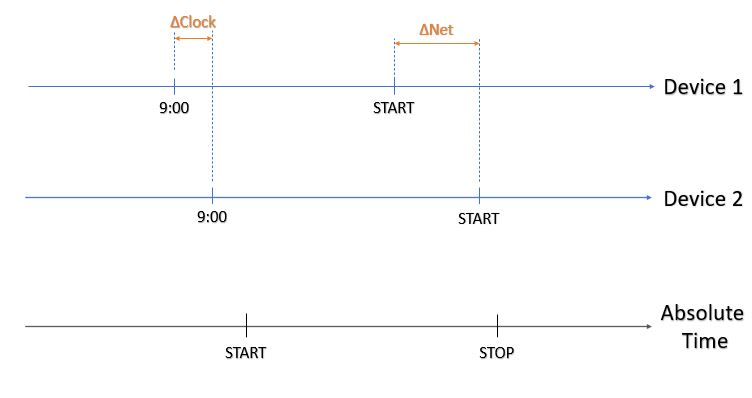
\includegraphics[width = 12cm]{FIGURAS/ejes_temporales.JPG}
\caption{Retardos de red y reloj}
\end{figure}


Los retardos mencionados se ilustran en la \textit{Figura 5.1}, donde se ha ejemplificado el retardo correspondiente a los relojes y el retardo correspondiente a la red, para dos dispositivos. También, en el tercer eje temporal de la figura, se muestra el resultado que se busca, es decir, un eje de tiempos absoluto, donde solo existe el retardo correspondiente al tiempo de propagación.

Conociendo el retardo que hay que eliminar, se logrará una serie de señales con un eje temporal absoluto y únicamente con el retardo físico producido por la propia transmisión de las señales desde el altavoz hasta los micrófonos de los dispositivos. El propósito de este capítulo es hallar de la forma más exacta posible este retardo comentado. Se propondrá dos alternativas de sincronización distintas.


\section{Correlación cruzada}
En procesado de señales, la correlación cruzada es de gran utilidad, ya que es una herramienta matemática que proporciona la relación entre dos señales, pudiendo llegar a medir el grado de similitud entre señales. Su procedimiento se basa en la convolución de una de las señales con la otra invertida.

\begin{equation}
R_{x,y}[k] = \sum_{k = -\infty}^{\infty} x[k] y[k-n]
\end{equation}

La correlación cruzada de una señal con ella misma es llamada autocorrelación. Un ejemplo de autocorrelación de una señal contaminada con ruido de media la unidad se muestra en la \textit{Figura 5.1}.

\begin{figure}[hbtp]
 \centering
 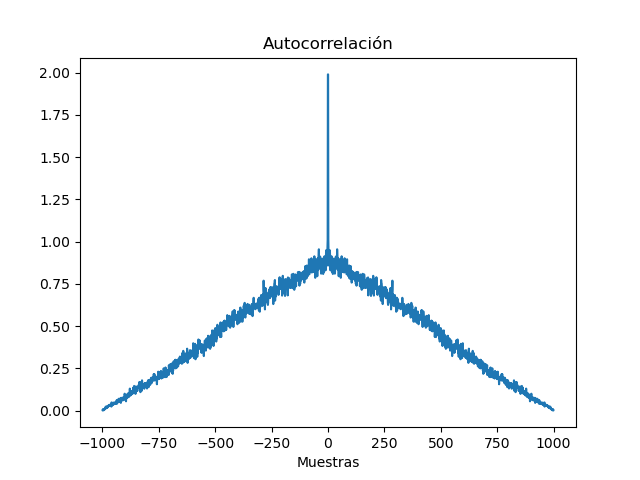
\includegraphics[width = 10cm]{FIGURAS/autocorrelacion.png}
 \caption{Autocorrelación}
 \end{figure}

La correlación cruzada será máxima en el instante de llegada de la señal. Como en la \textit{Figura 5.1} se está computando la misma señal, el máximo de la correlación se sitúa en 0 muestras, ya que no existe retardo alguno.

Para la correlación cruzada de dos señales con la diferencia de un intervalo de tiempo no conocido, el máximo de la correlación señalará el tiempo de llegada de una de las señales, es decir, el retardo que se busca para la sincronización de las señales.

\section{Señales de sincronización}
Se necesita conocer el desfase entre señales de la forma más precisa posible. Para ello, se proponen varias señales ejemplo, con el fin de obtener un máximo de correlación coherente.

La idea es introducir en la grabación creada por los dispositivos, una primera parte formada por señales de sincronización, con el fin únicamente de hallar el desfase entre señales y, posteriormente, realizar el procesado correspondiente a beamforming. Se proponen diferentes señales ejemplo para implementar la sincronización comentada.

\subsubsection{Impulso}
Dentro de las señales discretas más utilizadas se encuentra el impulso unitario. El cual es utilizado para evaluar todo tipo de canales mediante la respuesta impulsiva. Se define un conjunto de muestras nulas excepto en 0 que toma un valor máximo de 1.
\[
\delta(n)=\left\lbrace\begin{array}{c} 1~si~n = 0 \\ 0~resto \end{array}\right.\]

Para el caso acústico y la transición que debe hacer la señal desde que el servidor manda reproducir la señal y esta se reproduce por el altavoz, el impulso unitario es demasiado ideal, por lo que se ha adaptado a un impulso desplazado a la derecha y con un total de 10 muestras que toman el valor máximo, ya que si se hace más ideal el impulso no es reproducido correctamente.

\begin{figure}[hbtp]
\centering
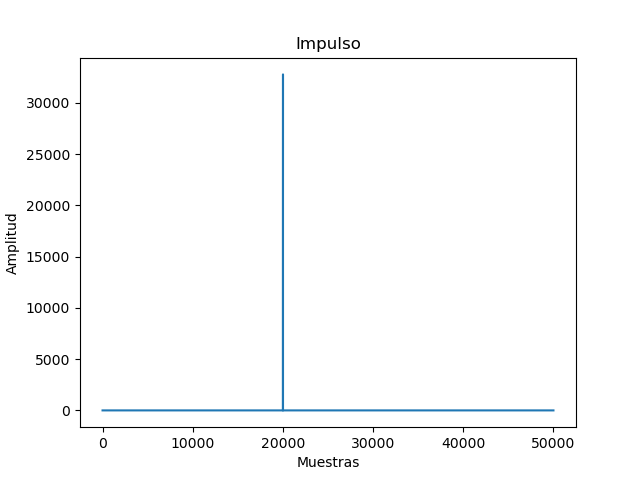
\includegraphics[width = 10cm]{FIGURAS/impulso.png}
\caption{Señal impulsiva}
\end{figure}


La señal creada se muestra en la Figura 5.2

\subsubsection{Chirp}
Un ''chirp'' es un tipo de señal con una variación determinada de la frecuencia instantánea. Un chirp hace un barrido entre dos frecuencias asignadas, de forma que la correlación cruzada entre dos señales ''chirp'' iguales, será máxima al detectar estas variaciones en frecuencia en los instantes de tiempo correspondientes al chirp original.

Se ha creado un chirp el cual hace un barrido en frecuencia entre 5000 y 16000 Hz y una duración total de 0.1 segundos, la cual ha sido la duración mínima para su correcta reproducción y función requerida. Un ''zoom'' de la señal comentada se presenta en la Figura 5.3, donde se puede observar el cambio en la frecuencia instantánea.

\begin{figure}[hbtp]
\centering
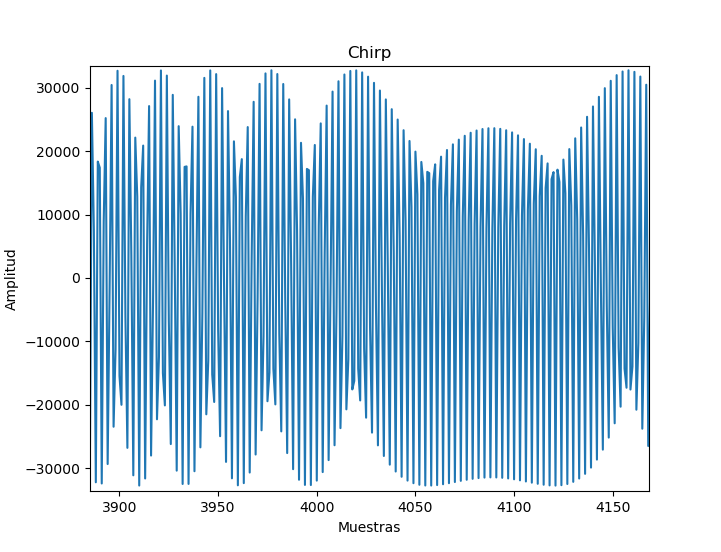
\includegraphics[width = 10cm]{FIGURAS/chiirp.png}
\caption{Chirp creado}
\end{figure}


A parte de ser utilizado el chirp para sincronizar señales y obtener un valor de correlación óptimo, es altamente utilizado en comunicaciones ópticas. El método que se menciona es conocido como \textit{prechirping} y consiste en una modificación de las características del pulso antes de ser introducido en una fibra óptica. En la \textit{Figura 5.4} se aprecia un pulso gaussiano sin modificar y un pulso gaussiano con chirp.

\begin{figure}[hbtp]
\centering
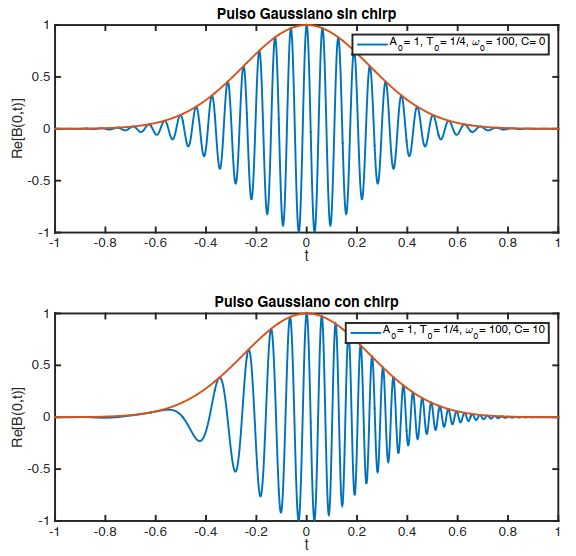
\includegraphics[width = 9cm]{FIGURAS/chirp.JPG}
\caption{Prechirping}
\end{figure}


Esta compensación previa puede hacer que el pulso se comprima y alcanzar longitudes de enlace de la fibra mayores e incluso  transmisiones con mejor detección en el receptor, como justifica \textit{[X]}.
\subsubsection{Tren de impulsos}
Como última señal, se propone un tren de impulsos. Consta de la concatenación de varios impulsos seguidos. De este modo, se consigue que, al realizar la operación de correlación cruzada, tengan que coincidir cada impulso con su correspondiente mientras se realiza la convolución, siendo máxima la correlación en el instante en que todos los impulsos coincidan.

\begin{figure}[hbtp]
\centering
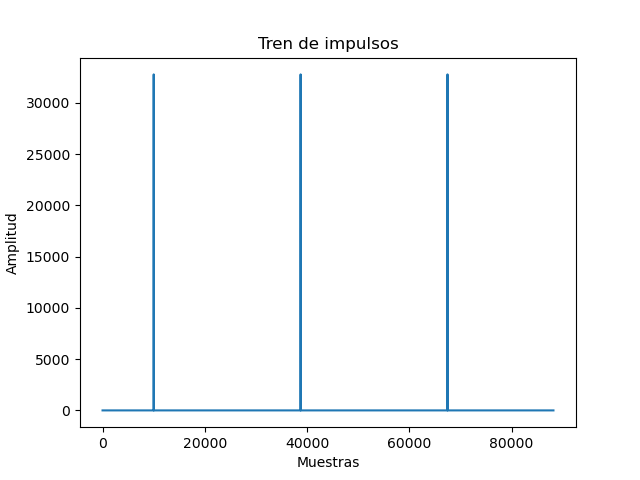
\includegraphics[width = 9cm]{FIGURAS/tren_impulsos.png}
\caption{Tren de impulsos}
\end{figure}

Analizadas las tres variantes de señal de sincronización propuestas, se procede a explicar dos métodos de sincronización distintos.

Se ha creado un tren de un total de tres impulsos, siendo estos equidistantes y teniendo en cuenta un margen de muestras inicial y final para la correcta reproducción por el altavoz y captación por los móviles. La señal comentada es representada en la \textit{Figura 5.4}.



\section{Sincronización mediante el servidor}

El primer método de sincronización propuesto, es realizado mediante la ayuda externa del servidor. Se conoce que, las marcas temporales de los móviles no son muy fiables, ya que arrastran el retardo debido a los relojes, por lo que se llega a la idea de que el servidor emita una señal de sincronización cuando todos y cada uno de los móviles estén en estado activo de grabación.

Cuando el servidor recibe la confirmación de cada dispositivo de haber comenzado a grabar, procede a la reproducción, por un altavoz monofónico, de una señal acústica la cual servirá de referencia para cada dispositivo. La idea es que la señal de sincronización comentada, sea grabada por todos los móviles y, acto seguido, sin detener la grabación, captar una segunda señal o señal principal. Esta última señal, es la que se debe obtener sin retardo alguno de red y la que se debe transmitir para realizar el proceso de beamforming.

De forma ideal, se deberán sincronizar todas las  $N$ señales de forma perfecta con un retardo nulo. Esto se pretende conseguir realizando un análisis mediante correlación cruzada de la señal acústica de sincronización captada por primera vez por uno de los dispositivos y esta misma señal grabada por los demás dispositivos. De esta manera, se supone el tiempo inicial 0 en el instante en que uno de los dispositivos capta primero la señal de sincronización. Como se ha comentado en la sección anterior, el mayor pico resultante de la correlación cruzada, corresponderá en muestras, al retardo de la señal grabada respecto a la señal primera.

\subsection{Análisis}
Antes de hablar de retardos y modificaciones en las grabaciones, se debe elegir la señal de sincronización.

\begin{figure}[hbtp]
\centering
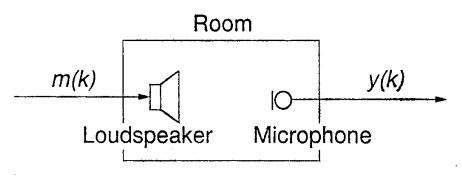
\includegraphics[width = 9cm]{FIGURAS/altavoz-micro.JPG}
\caption{Bloque altavoz-micrófono}
\end{figure}


Se realizaron diversas pruebas para cada una de las señales propuestas en la sección anterior. Hay que tener en cuenta que, al usar un altavoz externo para emitir la señal de sincronización, como en la \textit{Figura 5.7}, se pueden producir efectos no deseados, como modificaciones no controladas de la señal a la salida del altavoz. Este efecto se conoce como distorsión no lineal y puede producir error en las medidas. Haciendo referencia los estudios de \textit{[X]}, el error causado por distorsión no lineal aparece como pulsos aleatoriamente distribuidos pero espaciados una distancia similar a la del período de muestreo (\textit{Figura 5.8.a}). Este efecto no lineal se puede disminuir bajando el nivel de sonido del altavoz (\textit{Figura 5.8.b}), sin embargo, si se disminuye demasiado, el ruido de fondo llega a tener un impacto considerable en la señal de interés y se incrementa el error aleatorio (\textit{Figura 5.8.c}).

\begin{figure}[hbtp]
\centering
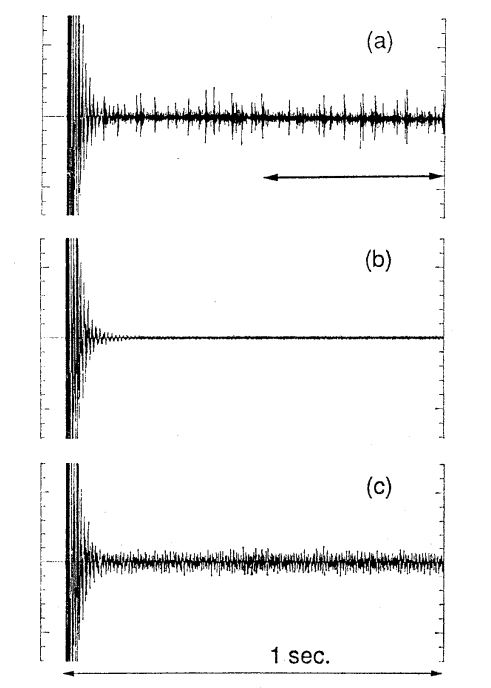
\includegraphics[width = 8cm]{FIGURAS/nonlinear.JPG}
\caption{Efecto de la no-linealidad}
\end{figure}

Realizando pruebas de sincronización con la señal del tipo ''chirp'', no se llegaba a obtener una buena correlación. Con buena correlación se entiende como un máximo de correlación preciso y distinguible. Esta poca precisión desembocó en un retardo final inadmisible. Este resultado no tan bueno con la señal de sincronización chirp puede ser debido a los efectos no lineales producidos por el altavoz, ya que los chirps son muy utilizados para procesos de sincronización por los cambios en la frecuencia instantánea de la señal, los cuales son clave para correlar muestras. A pesar de esto, si no se capta bien estas modificaciones en frecuencia en el instante preciso, la correlación cruzada puede resultar errónea.

Habiendo tomado la decisión de no utilizar el chirp, se probó con la señal impulso. Se obtuvieron mejores resultados.

Por último, se experimentó la sincronización con el tren de impulsos, obteniendo la máxima precisión en el máximo de la correlación de las tres señales, por lo que se ha optado en este método por el uso del \textbf{tren de impulsos} como señal de sincronización acústica.

\subsection{Procedimiento}

Con el propósito de tomar de referencia el primer tiempo de llegada de la señal de sincronización, se debe determinar cuál es el dispositivo que capta primero esta señal. Con este dato, se fijará el instante cero en la grabación de este dispositivo y se buscará los retardos respecto a este instante.

Para determinar la primera captación de la señal de sincronización, se emplea la correlación cruzada del tren de impulsos creado y del tren de impulsos captado en la grabación de cada uno de los dispositivos. Una vez conocida la grabación de referencia, se realiza de nuevo un análisis de correlación cruzada, entre el tren de impulsos de la grabación de referencia y el tren de impulsos de cada uno de los dispositivos. El máximo valor de las $N$ correlaciones cruzadas coincide con el retardo correspondiente en función del instante de referencia.


\begin{figure}
 \centering
  \subfloat[]{
   \label{autocorr}
    \includegraphics[width=7cm]{FIGURAS/correlacion_misma_señal.png}}
  \subfloat[]{
   \label{correlaimpulsos}
    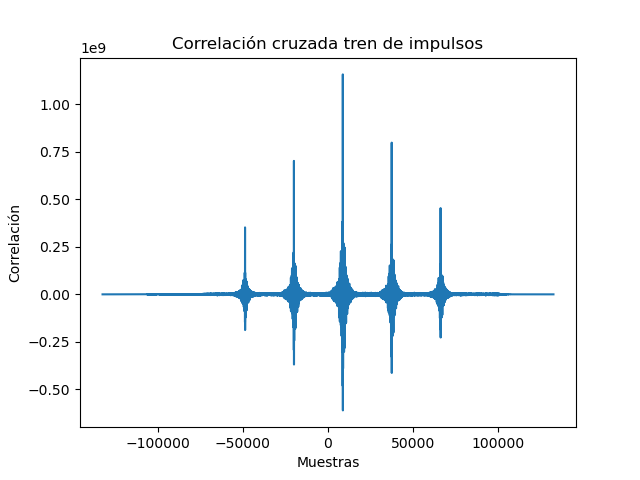
\includegraphics[width=7cm]{FIGURAS/correlacion_tren.png}}
 \caption{Correlaciones tren de impulsos}
\end{figure}

En la figura \ref{autocorr} se muestra la autocorrelación entre la señal tren de impulsos de la grabación de referencia tomada. Trivialmente, en este caso el retardo es cero exacto. Se pueden 4 máximos locales y un máximo absoluto en la traza de la correlación. Los máximos locales se corresponden a la superposición de los impulsos en el proceso del desplazamiento de la señal en la convolución con la señal invertida. Cuando se superponen todos y cada uno de los impulsos, las dos señales están perfectamente cuadradas y se produce el máximo absoluto, el cual muestra el retardo de una señal respecto a la otra.

La correlación cruzada entre el tren de impulsos del dispositivo tomado como referencia temporal y el tren de impulsos grabado por otro dispositivo diferente se presenta en la figura \ref{correlaimpulsos}. Se observa que el máximo absoluto posee una cierta desviación respecto al 0 en el eje de abcisas. El valor de este máximo se corresponde con el retardo de la grabación de este smartphone.

Conocido el retardo de cada grabación, se procede a eliminar las muestras correspondientes, acortando cada señal desde el principio. Debido a que la orden de parar la grabación no llega en el mismo instante para todos los móviles, las señales se deberán acortar también por el final, determinando el tamaño para todas las grabaciones como la longitud mínima de todas las señales una vez acortadas las muestras correspondientes al retardo inicial. Mediante este proceso de eliminación de muestras inferiores y superiores, se obtiene una matriz con todas las grabaciones sincronizadas con un mismo número de muestras.

\begin{figure}
 \centering
  \subfloat[]{
   \label{sincro_server}
    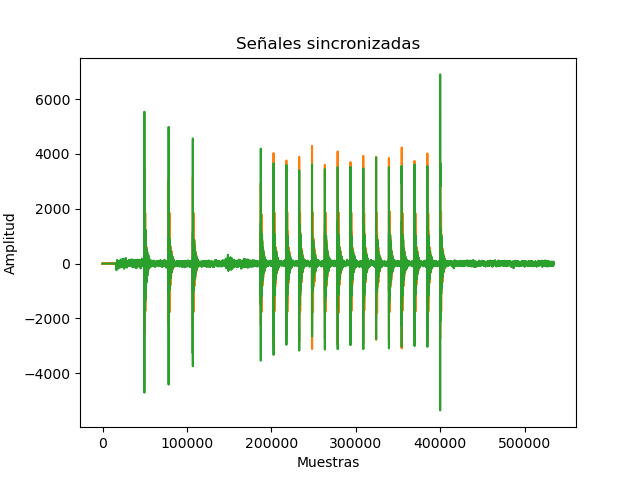
\includegraphics[width=7cm]{FIGURAS/sincro_server.png}}
  \subfloat[]{
   \label{correla_sincroniz}
    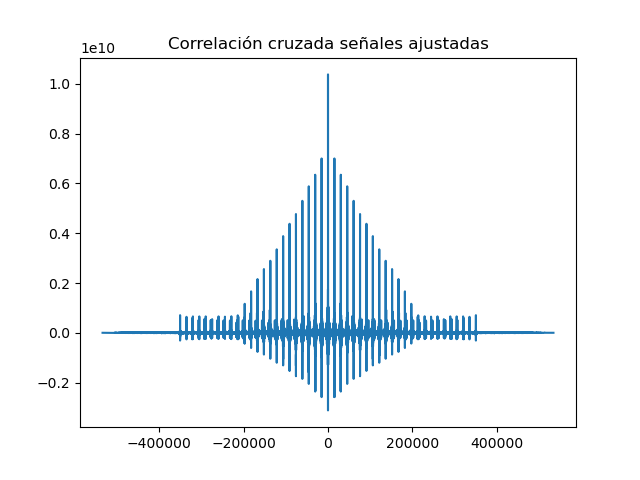
\includegraphics[width=7cm]{FIGURAS/correla_sincronizadas.png}}
 \caption{Señales sincronizadas}
\end{figure}



En la figura \ref{sincro_server} las señales perfectamente sincronizadas. En el caso de la simulación, se ha realizado la sincronización con 3 dispositivos. Su comprobación se puede consultar en la figura \ref{correla_sincroniz} donde se muestra una correlación cruzada entre la grabación de un dispositivo y la grabación de otro dispositivo distinto. Anotar que, la señal principal se corresponde con un tren de impulsos de 15 impulsos en total, por eso la correlación cruzada de la figura \ref{correla_sincroniz} posee esos picos tan uniformemente separados.



\section{Sincronización mediante ''auto-chirps''}
\section{Análisis comparativo}


\chapter{Implementación del algoritmo de Beamforming}

\chapter{Análisis del modelo}

\chapter{Perspectiva de futuro}
Aquí poner lo del 5G, massive MIMO etc Y ALGUNA COSA MÁS.
\chapter{Conclusiones}

\chapter{Bibliografía}



\chapter{Apéndice}





%\input{capitulos/01_Introduccion}
%
%\input{capitulos/02_EspecificacionRequisitos}
%
%\input{capitulos/03_Planificacion}
%
%\input{capitulos/04_Analisis}
%
%\input{capitulos/05_Diseno}
%
%\input{capitulos/06_Implementacion}
%
%\input{capitulos/07_Pruebas}
%
%\input{capitulos/08_Conclusiones}
%
%%\chapter{Conclusiones y Trabajos Futuros}
%
%
%%\nocite{*}
%\bibliography{bibliografia/bibliografia}\addcontentsline{toc}{chapter}{Bibliografía}
%\bibliographystyle{miunsrturl}
%
%\appendix
%\input{apendices/manual_usuario/manual_usuario}
%%\input{apendices/paper/paper}
%\input{glosario/entradas_glosario}
% \addcontentsline{toc}{chapter}{Glosario}
% \printglossary
\chapter*{}
\thispagestyle{empty}

\end{document}
